\documentclass{report}
\author{Ben Haladik}
\title{Bioinformatische Anwendung von \textit{Graphlets} zur Analyse von Proteinstrukturtopologien \\ Rohfassung}
\usepackage{mathtools}
\usepackage{amsfonts}
\usepackage{ngerman}
\usepackage{hyperref}
%\usepackage{natbib}
\usepackage{rotating}
\usepackage[table, dvipsnames, usenames]{xcolor}
\usepackage{color}
\usepackage[justification=centering]{caption}
\usepackage{float}
\usepackage{subcaption}
\usepackage[linesnumbered,lined,boxed,commentsnumbered, ngerman]{algorithm2e}
%\usepackage{qtree}
%\usepackage{cite}
\definecolor{fGreen}{rgb}{0.13,0.54,0.13}
\usepackage{caption}
\usepackage{array}
\usepackage{acronym}
\newcolumntype{C}[1]{>{\centering\let\newline\\\arraybackslash\hspace{0pt}}m{#1}}

\setlength{\parindent}{0.5em}



\begin{document}

\definecolor{green}{rgb}{0.13,0.54,0.13}


\maketitle

\newpage

\tableofcontents

\newpage

\listoffigures

\newpage



\listoftables

\newpage

\bigskip
\begin{Huge}
\textbf{Abk\"urzungsverzeichnis}
\end{Huge}

\vspace{15mm}
\begin{acronym}
\acro{PDB}{\textit{Protein Data Bank}}
\acro{PTGL}{\textit{Protein Topology Graph Library}}
\acro{RGF}{Relative \textit{Graphlet} H\"aufigkeiten Distanz}
\acro{SSE}{Sekund\"arstrukturelement}
\end{acronym}


\newpage

\chapter{Einleitung}

\section{Motivation}


Proteine sind die essentiellen Bausteine zellul\"aren Lebens. Jede Aktivit\"at eines Organismus kann durch die Aktivit\"at der beteiligten Proteine beschrieben werden. Dementsprechend ist ein tiefes Verst\"andnis von Proteinen zentral f\"ur das Verst\"andnis von zellul\"arem Leben.
Die Struktur eines Proteins bestimmt seine Funktion und die vergleichende Analyse dieser Strukturen liefert Einblicke in entfernte evolution\"are Verwandschaftsbeziehungen, die durch reine Sequenzanalysen nicht mehr nachvollziehbar sind.

Hierzu betrachten wir Proteinstrukturtopologien. Die Topologie eines Proteins ist als die Anordnung seiner Sekund\"arstrukturelemente (SSEe)
 zueinander definiert. Die Betrachtung von SSEe hat den Vorteil, dass diese auch \"uber gro"se evolution\"are Distanzen stark konserviert sind. Es ist also naheliegend, Proteine entsprechend ihrer Topologien einzuordnen.

Da die Anzahl der bekannten Proteinstrukturen in den letzten Jahren rasant angestiegen sind, ist es nicht mehr m\"oglich diese Einordnung und die hierf\"ur n\"otigen Vergleiche nur manuell vorzunehmen. Es werden algorithmische Vergleichsmethoden und entsprechende Datenstrukturen ben\"otigt.

Zur Darstellung dieser Topologien werden hier Graphen verwendet. Graphen geh\"oren zu den am st\"arksten untersuchten mathematischen Strukturen, da sich mit ihnen viele verschiedene komplexe Zusammenh\"ange darstellen lassen. Ihre Nutzung ist \"uberall dort angebracht, wo Daten nicht als Zahlen oder Vektoren darstellbar sind, weil sie eine Menge von Objekten und ihre Beziehungen untereinander repr\"asentieren.


Graphen finden sich in der Erforschung von sozialen Netzwerken wieder und werden in der Chemie zur Darstellung von Molek\"ulen genutzt. Auch in der Bioinformatik sind Graphen das zentrale Mittel zur Darstellung komplexer Beziehungen. Interaktionen von Proteinen werden genauso als Graphen modelliert, wie Signalwege in Zellen oder eben Proteine. Die Analyse von biologischen Netzwerken ist ein zentrales Mittel, um biologische Vorg\"ange besser zu verstehen \cite{junker2011analysis}.

Der Vergleich von Graphen ist jedoch keine triviale Aufgabe. Die Frage: "`Ist dieser Graph in diesem anderen Graphen enthalten?"' befriedigend schnell beantworten zu k\"onnen, ist nicht m\"oglich, denn das zugrunde liegende Entscheidungsproblem ist NP-vollst\"andig \cite{karp1972reducibility}.

Um dieses Problem zu umgehen, werden approximative Methoden angewandt. Hierzu geh\"ort das Berechnen von \textit{Graphlets} \cite{frqdistribution}. \textit{Graphlets} sind kleine, induzierte Teilgraphen, die f\"ur gro"se Graphen immer noch schnell abz\"ahlbar sind. Mit dieser Technik lassen sich in polynomieller Zeit Teilstrukturen eines Graphen ermitteln. Dabei erh\"alt man Vektoren, deren Vergleich einfacher durchzuf\"uhren ist, als ein direkter Vergleich der Graphen selbst. So lassen sich \textit{Graphlets} zur vergleichenden Analyse von Proteinstrukturtopologien verwenden.




\section{\textit{State of the art}}

Mit der wachsenden Anzahl von Struktureintr\"agen in der \textit{Protein Data Bank} (PDB) ist eine Vielzahl von Methoden entstanden, um diese Strukturen zu vergleichen.

Der wohl bekannteste Algorithmus zum Vergleich von dreidimensionalen Proteinstrukturen ist DALI von \textit{Holm} und \textit{Sander} \cite{holm1993protein}. Er f\"uhrt ein globales Alignment durch, indem Distanzmatrizen verglichen werden. In diesen Matrizen sind die intramolekularen Distanzen der $C_\alpha$-Atome der jeweiligen Proteine eingetragen.

In den 23 Jahren, die seit der Ver\"offentlichung von DALI vergangen sind, sind aber noch viele weitere Methoden mit unterschiedlichen Ans\"atzen entwickelt worden. Der Algorithmus von \textit{Shindyalov} und \textit{Bourne} \cite{shindyalov1998protein} berechnet ein Alignment von Proteinstrukturen, indem er zun\"achst kleine Paare von Substrukturen aligniert und dann versucht, dieses Alignment auf einen optimalen Pfad auszudehnen.

Der FATCAT-Algorithmus von \textit{Ye} und \textit{Godzik} \cite{fatcat} verwendet eine \"ahnliche Idee und versucht zus\"atzlich, die Substrukturen flexibel zu alignieren, um auch gleiche Proteine mit ver\"anderter Konformation erkennen zu k\"onnen.

\textit{TM-align} von \textit{Zhang} und \textit{Skolnick} \cite{zhangtm} berechnet eine Rotationsmatrix und nutzt Dynamische Programmierung. Der Algorithmus benutzt als Bewertungsschema den sogenannten \textit{TM-Score}, der besonders gut geeignet ist, um lokale \"Ahnlichkeiten zu erkennen.

Der SSM-Algorithmus von \textit{Krissinel} und \textit{Hendrick} \cite{pdbefold} verwendet eine graphenbasierte Darstellung von Proteinen f\"ur ein erstes Alignment und verfeinert dieses dann durch die Berechnung der Distanzen \"aquivalenter $\alpha$-C-Atome. Er wird im \textit{PDBeFold-Web-Server} implementiert. Als einziger hier beschriebener Algorithmus erm\"oglicht er schnelle multiple Strukturvergleiche \"uber einen \textit{Web-Service}.


Die meisten dieser Methoden f\"uhren einen \textit{Template}-basierten Vergleich durch. Das hei"st, dass der \"Ahnlichkeitswert, der einem Paar zugewiesen wird, zum einen von der Reihenfolge der Eingabe abh\"angt und zum anderen von den Proteinen abh\"angt, die Teil des multiplen Vergleichs sind, aber nicht zu dem gerade betrachteten Paar geh\"oren.
Als \"Ahnlichkeitswerte werden paarweise durchschnittliche Abst\"ande der Strukturen zueinander ausgegeben.


Im Gegensatz zu diesen rein algorithmischen Methoden verwenden Datenbanken wie CATH \ref{cath} und SCOPe \ref{scope} eine Mischung aus algorithmischen Methoden und manueller Einordnung durch Experten, um Proteine in strukturelle Klassen einzuordnen.

\textit{Graphlets} wurden zuerst von \textit{Pr{\v z}ulj et al.} auf biologische Daten angewandt \cite{frqdistribution}, \cite{graphletfrequency}. Sie nutzten den \textit{Graphlet}-Algorithmus, um \"Ahnlichkeiten von Protein-Protein-Interaktionsnetzwerken zu berechnen.

\textit{N. Shervashidze} war die erste, die \textit{Graphlets} zur Analyse von Proteinstrukturen anwandte \cite{sherv_graphlets}. Sie nutzte \textit{Support Vector Machines} mit \textit{Graphlet}-Vektoren, um  f\"ur Proteingraphen zu entscheiden, ob diese Enzyme darstellen oder nicht.

Auch von \textit{Tatiana Bakirova} wurden \textit{Graphlets} verwendet, um Proteinstrukturen zu analysieren \cite{bakirova2013comparison}. Sie hat das Programm \texttt{graphletAnalyser} verfasst, das in dieser Arbeit genutzt und weiterentwickelt wurde.

\section{Ziele}

Ziel dieser Arbeit war zun\"achst die Erweiterung der Funktionalit\"at von \\ \texttt{graphletAnalyser}. Hierzu geh\"ort zun\"achst eine funktionierende Datenbankanbindung, um die berechneten Daten abzuspeichern. Die Ausgabe sollte so erweitert werden, dass das Berechnen der Verteilungen der relativen H\"aufigkeiten der \textit{Graphlets} m\"oglich wird.
Das Berechnen von markierten \textit{Graphlets} sollte so implementiert werden, dass es auf Graphen mit beliebigen Markierungen angewandt werden kann. Deshalb wurde ein Algorithmus entwickelt und implementiert, der aus einem Alphabet von Knotenmarkierungen alle Worte berechnet, die markierte  2- und 3-\textit{Graphlets} repr\"asentieren -- der \textit{Graphlet}-Worte-Algorithmus. Die Suche nach diesen markierten \textit{Graphlets} in einem Graphen wurde ebenfalls implementiert.


In Fallstudien wird \"uberpr\"uft, ob und inwiefern sich \textit{Graphlets} eignen, um die \"Ahnlichkeit von Proteinstrukturtopologien zu untersuchen. Dies wurde mit unterschiedlichen Metriken getestet. Die hierbei errechneten \"Ahnlichkeitswerte wurden mit den Ergebnissen des Strukturalignment-Programms \textit{PDBeFold} \cite{pdbefold} verglichen.


Weiterhin wurde untersucht, wie die relativen H\"aufigkeiten der \textit{Graphlets} in einem gro"sen Faltungsraum verteilt sind. Um zu \"uberpr\"ufen, ob sich Superfamilien anhand dieser Verteilungen voneinander abgrenzen lassen, wurden diese H\"aufigkeiten f\"ur den PDBTop500-Datensatz mit einem Datensatz aus Aldolasen verglichen.



\section{Aufbau der Arbeit}

Zun\"achst wird im Kapitel \emph{Materialien und Methoden} die \textit{Protein Topology Graph Library} (PTGL) \cite{ptgl1} vorgestellt, deren Idee die Grundlage f\"ur diese Arbeit liefert. 
 
Es folgt eine Kurzbeschreibung von PLCC, der \textit{Software}, die die Graphen der PTGL erstellt und diese verwaltet, sowie eine Beschreibung des \textit{Graphlet}-Algorithmus.

Weiterhin wird das Programm \texttt{graphletAnalyser} vorgestellt, welches den \textit{Graphlet}-Algorithmus implementiert.
Anschlie"send wird die erste Metrik vorgestellt, mit denen die erhaltenen \textit{Graphlet}-Vektoren verglichen werden. Es folgt eine Beschreibung der verwendeten Datens\"atze und von \textit{PDBeFold}, dessen Ergebnisse mit denen von \texttt{graphletAnalyser} verglichen werden.

Im Ergebnisteil wird zun\"achst der modifizierte Jaccard-Index pr\"asentiert, der sich mit leichten \"Anderungen am Tanimoto-Koeffizienten orientiert. Dann folgen Beschreibungen des neuen \textit{Graphlet}-Worte-Algorithmus und der in den Fallstudien erhaltenen Ergebnisse.

Im abschlie"senden Teil \emph{Diskussion und Ausblick} wird versucht, die Frage zu kl\"aren, ob sich \textit{Graphlets} f\"ur multiplen Proteinstrukturvergleich und \"ahnliche Anwendungen eignen. Weiterhin wird untersucht, ob Modifikationen der \textit{Graphlet}-Vektoren, oder der Metriken n\"otig sein k\"onnten, um bessere Ergebnisse zu erhalten. 



\chapter{Materialien und Methoden}






\section{\textit{Protein Topology Graph Library}}


Die \textit{\underline{P}rotein \underline{T}opology \underline{G}raph \underline{L}ibrary} entstand aus einer Idee von \textit{Patrick May} und \textit{Ina Koch} \cite{ptgl1}. Ausgehend von der Tatsache, dass sich Proteinstrukturtopologien als r\"aumliche Beziehungen von SSEen untereinander definieren lassen, verwendet die PTGL \emph{Graphen}, um Proteinstrukturtopologien darzustellen.
Hierbei stellen die Knoten des Graphen die SSEe eines Proteins dar. Sie werden dem jeweiligen SSE entsprechend markiert. Knoten, die $\alpha$-Helices repr\"asentieren, werden mit einem H markiert, $\beta$-Faltbl\"atter mit einem E. Weiterhin erm\"oglicht die PTGL die Darstellung von Liganden, \cite{vplg} denen mit L markierte Knoten zugeordnet werden. Um die r\"aumliche Nachbarschaft von SSEs und Liganden mit- und untereinander darstellen zu k\"onnen, werden ungerichtete Kanten zwischen Knoten gezogen, wenn die entsprechenden Elemente benachbart sind. Jede Polypeptidkette eines Proteins wird dann als \emph{Proteingraph} dargestellt. Die Zusammenhangskomponenten eines Proteingraphen werden als Faltungsgraphen bezeichnet, weil sie typischerweise eine unabh\"angige Faltungseinheit darstellen.

Durch diese abstrahierte Darstellung k\"onnen zentrale Charakteristika eines Proteins wie Motive und Dom\"anen einfach visualisiert werden.


\section{PLCC}

PLCC ist die \textit{Software}, die die Daten der PTGL generiert und verwaltet. Sie wurde von \textit{Tim Sch\"afer} geschrieben und  wird von ihm verwaltet.


\paragraph{Die Berechnung der Graphen der PTGL}

erfolgt unter Verwendung der entsprechenden PDB- und DSSP-Dateien. Um den Graphen f\"ur eine Polypeptidkette zu berechnen, werden aus der DSSP-Datei die SSEe des Proteins ausgelesen. F\"ur jedes Paar von SSEs wird die Anzahl der r\"aumlichen Kontakte ihrer Residuen in der PDB-Datei berechnet. Wenn die Anzahl dieser Kontakte einen gewissen Grenzwert \"uberschreitet, wird angenommen, dass diese SSEs r\"aumlich benachbart sind und die jeweiligen Knoten werden durch eine Kante verbunden. So wird f\"ur jede Polypeptidkette ein Graph erstellt.

\paragraph{Komplexgraphen}

werden ebenfalls in dieser Arbeit untersucht. Ihre Berechnung erfolgt analog zur Berechnung der Proteingraphen. Der Unterschied besteht darin, dass ein Komplexgraph mehrere Polypeptidketten beschreibt.

\paragraph{Aminos\"auregraphen} werden analog zu Proteingraphen und Komplexgraphen berechnet. Der Unterschied zu den anderen Graphformaten ist, dass keine SSEs betrachtet werden. Stattdessen repr\"asentiert jeder Knoten eine Aminos\"aure eines Proteins. Die Knoten werden entsprechend der chemischen Eigenschaften der Aminos\"auren markiert. Knoten, die saure oder basische Aminos\"aurenreste darstellen, werden mit einem c markiert. Ein p markiert Knoten als polare Reste, die weder sauer noch basisch sind. F\"ur unpolare Aminos\"auren wird ein h verwendet. Auch Liganden k\"onnen in Aminos\"auregraphen dargestellt werden. Ihre Knoten werden durch ein ? markiert. Aminos\"auregraphen k\"onnen Proteinkomplexe und einzelne Polypeptidketten darstellen.


Weiterhin erm\"oglicht PLCC den Vergleich von \textit{Graphlet}-Vektoren, die im folgenden Teil vorgestellt werden.


\section{Der \textit{Graphlet}-Algorithmus}


Um diese Graphen vergleichen zu k\"onnen, werden \textit{Graphlets} verwendet. Diese sind im Gegensatz zu Graph-Isomorphismen in polynomieller Zeit berechenbar \cite{sherv_graphlets}. \textit{Graphlets} sind kleine, induzierte Teilgraphen mit bis zu f\"unf Knoten. Die Abbildungen \ref{fig:3graphlets}, \ref{fig:4graphlets} und \ref{fig:5graphlets} zeigen die \textit{Graphlets} mit drei, vier und f\"unf Knoten. Wir betrachten hierbei ausshlie"lich die zusammenh\"angenden \textit{Graphlets}. Sie werden durch den Algorithmus gez\"ahlt und ihre jeweilige relative H\"aufigkeit wird in einen Vektor geschrieben, den wir als \textit{Graphlet}-Vektor bezeichnen.


\subsection{Beschreibung des Algorithmus}
Um alle \textit{Graphlets} der Gr\"o"se $k \in \{3,4,5\}$ zu z\"ahlen, werden alle Euler-Wege der L\"ange $k-1$ in dem gegebenen Graphen gesucht. F\"ur jeden gefundenen Euler-Weg werden alle inzidenten Kanten aller Knoten des Weges \"uberpr\"uft. Wird hierbei ein \textit{Graphlet} gefunden, wird der Z\"ahler f\"ur das entsprechende \textit{Graphlet} im \textit{Graphlet}-Vektor um den Wert an der entsprechenden Stelle der unten stehenden Gewichtungsvektoren $w_k$ erh\"oht.


F\"ur \textit{Graphlets} mit $k \geq 4$ existieren zus\"atzlich die sogenannten Stern-\textit{Graphlets}. Das sind $g_4$ in \ref{fig:4graphlets}, sowie $g_{19}$,$g_{20}$ und $g_{21}$ in \ref{fig:5graphlets}. Diese enthalten keinen solchen Euler-Weg.

\begin{center}
\begin{subequations}
\label{eq:w-vector}
\begin{align*}
\text{\textit{Graphlet}-Gewichtungsvektoren} \\
w_2 := \left( \frac{1}{2} \right) \\
w_3 := \left( \frac{1}{6}, \frac{1}{2} \right) \\
w_4 := \left( \frac{1}{24}, \frac{1}{12}, \frac{1}{4}, 1, \frac{1}{8},\frac{1}{2} \right) \\
w_5 := \left( \frac{1}{120}, \frac{1}{72}, \frac{1}{48}, \frac{1}{36}, \frac{1}{28}, \frac{1}{20}, \frac{1}{14}, \frac{1}{10}, \frac{1}{12}, \frac{1}{8}, \frac{1}{4}, \frac{1}{2}, \frac{1}{12} \frac{1}{12}, \frac{1}{4} \frac{1}{4}, \frac{1}{2}, 1, \frac{1}{2}, 1\right)
\end{align*}
\end{subequations}
\end{center}

Jede Stelle eines Gewichtungsvektors $w_k$ ist mit einem \textit{Graphlet} assoziiert. Die Nenner der Br\"uche in den Vektoren entsprechen den Anzahlen der Euler-Wege der L\"ange $k-1$ in den entsprechenden \textit{Graphlets}. Wenn alle Euler-Wege eines \textit{Graphlets} besucht wurden und der zugeh\"orige induzierte Teilgraph ihm entspricht, wird sein Z\"ahler im \textit{Graphlet}-Vektor ganzzahlig und das \textit{Graphlet} gilt als gefunden.
Hierbei bilden  die Stern-\textit{Graphlets}, die keine Euler-Wege der L\"ange $k-1$ enthalten, nat\"urlich die Ausnahme.
 
Da wir 29 verschiedene \textit{Graphlets} betrachten, hat ein \textit{Graphlet}-Vektor 29 Stellen. An jeder Stelle steht die relative H\"aufigkeit eines \textit{Graphlets}. Damit ist ein Vergleich in konstanter Zeit m\"oglich. Anstatt von Graphen oder dreidimensionalen K\"orpern werden mit diesem approximativen Verfahren Vektoren im Vektorraum $\mathbb{R}^{29}$ verglichen.



\section{\texttt{graphletAnalyser}}

In seiner urspr\"unglichen Version wurde das Programm bereits 2013 von \textit{Tatiana Bakirova} geschrieben. Im Sommer 2015 wurde es um einige Funktionen erweitert.

\texttt{graphletAnalyser} ist in C++ geschrieben. Zur internen Darstellung der Graphen wird die \textit{Boost-Graph-Library} verwendet. Die Anbindung an die \textit{Postgreql}-Datenbank wird mittels der Bibliothek pqxx realisiert.

\paragraph{Als Input} erh\"alt das Programm eine oder mehrere GML-Dateien, die Graphen darstellen. Aus jeder GML-Datei wird mit der \textit{Boost-Graph-Library} intern ein Graph erstellt, der f\"ur die Berechnungen verwendet wird.

F\"ur den eingelesenen Graphen berechnet das Programm alle \textit{Graphlets} mit drei, vier und f\"unf Knoten. Die Implementierung entspricht der \textit{Matlab}-Implementierung von \textit{N. Shervashidze} \cite{sherv_graphlets}. Zus\"atzlich berechnet es markierte \textit{Graphlets} der Gr\"o"sen 2 und 3, wobei die Markierungen den SSE-Zuordnungen der PTGL entsprechen. Es gibt 35 verschiedene markierte \textit{Graphlets} mit 2 oder 3 Knoten. Unter Ber\"ucksichtigung dieser Markierungen erh\"oht sich die Anzahl der Stellen der \textit{Graphlet}-Vektoren auf 64.
Die Knotengradverteilungen k\"onnen ebenfalls berechnet werden.

\paragraph{Der Output} des Programms umfasst zum einen die Ausgabe der \textit{Graphlet}-Vektoren mit oder ohne markierte \textit{Graphlets} in den Formaten csv, matlab und nova. Zus\"atzlich k\"onnen die \textit{Graphlet}-Vektoren in einer Datenbank, die zuvor mit PLCC erstellt wurde gespeichert werden. Die Knotengradverteilung kann zusammen mit anderen Daten eines Graphen als .csv-Datei ausgegeben werden.


\section{\"Ahnlichkeitsma"s}

Durch die Verwendung der \textit{Graphlets} wird der direkte Vergleich von Graphen durch einen Vergleich von \textit{Graphlet}-Vektoren ersetzt. Typischerweise wird eine eine Abstandsmessung durchgef\"uhrt, um Vektoren zu vergleichen. Hier verwenden wir eine Metrik von \textit{Pr\v{z}ulj et al.}.



\subsection{Relative \textit{Graphlet}-H\"aufigkeiten-Distanz}

\textit{Pr\v{z}ulj et al.} haben \textit{Graphlets} bereits auf Protein-Protein-Interaktionsnetzwerke (\cite{frqdistribution}) angewandt. Als Ma"s f\"ur die \"Ahnlichkeit von Netzwerken nutzen sie die Relative-\textit{Graphlet}-H\"aufigkeiten-Distanz (RGF). Diese Metrik berechnet den Abstand $D(G,H)$ zwischen zwei Graphen $G$ und $H$ als logarithmierte Differenz der normalisierten Anzahl der \textit{Graphlets} in $G$ und $H$. Sie ist folgenderma"sen definiert: \\

Sei $N_{i}(G)$ die Anzahl der \textit{Graphlets} von Typ $i \in {1,...,29}$ und \\ $T(G) = \sum_{i = 1}^{29} N_{i}(G)$ die Anzahl der \textit{Graphlets} in $G$, beziehungsweise $H$.\\

Dann ist $D(G,H)$ f\"ur zwei Graphen $G$ und $H$ definert als:

\begin{subequations}
\begin{align*}
D(G,H) := \sum_{i = 1}^{29} | F_{i}(G) - F_{i}(H) | \\
\text{mit } F_{i}(G) := - log(\frac{N_{i}(G)}{T(G)})
\end{align*}
\end{subequations}



Diese Metrik l\"asst sich analog zur euklidischen Distanz auffassen, denn sie berechnet den Abstand f\"ur zwei Vektoren $x,y$ als Differenz ihrer Eintr\"age $x_i -y_i$. Sie verwendet die normalisierten \textit{Graphlet}-Vektoren unter der Annahme, dass die \"Ahnlichkeit zweier Netzwerke sich aus der \"Ahnlichkeit lokaler Substrukturen ableiten l\"asst \cite{frqdistribution}. Somit k\"onnen Netzwerke, die \"ahnliche Substrukturen haben, sich aber in ihrer Gr\"o"se stark unterschieden, immer noch als \"ahnlich erkannt werden. Zus\"atzlich soll durch diese Normalisierung ausgeschlossen werden, dass einzelne besonders h\"aufige \textit{Graphlets} in einem Graphen die Messung verzerren.

Da alle Eintr\"age der Vektoren aus dem Intervall $ [0,1] \in \mathbb{R} $ stammen werden sie logarithmiert. Damit erh\"alt man Abst\"ande, die aus deutlich gr\"o"seren Intervallen stammen. Die Ergebnisse k\"onnen so leichter interpretiert werden und der Einfluss der Einfluss von Rundungsfehlern verkleinert sich. Dies sorgt auch daf\"ur, dass seltenere \textit{Graphlets} einen st\"arkeren Einfluss auf die Messung haben, als h\"aufige \textit{Graphlets}.
 
Weiterhin wurde gezeigt, (\cite{frqdistribution}) dass diese Metrik auch bei verrauschten Daten noch sehr gut funktioniert. Hierbei ist jedoch zu beachten, dass sie bisher vor allem f\"ur sehr gro"se Netzwerke mit mehreren Tausend Knoten und Kanten verwendet wurde. Diese Gr\"o"se kann von Aminos\"auregraphen erreicht werden, wenn sie gro"se Proteinkomplexe modellieren. Proteingraphen und Komplexgraphen sind aber deutlich kleiner.

\section{\textit{PDBeFold}}

Im Rahmen der Fallstudie wird \texttt{graphletAnalyser} mit \textit{PDBeFold} \cite{pdbefold} verglichen. \textit{PDBeFold} f\"uhrt ebenfalls einen graphenbasierten Strukrutvergleich durch. Analog zur PTGL modellieren Knoten SSEs. Zus\"atzlich werden diese mit der Anzahl von Residuen des jeweiligen SSE markiert. Im Gegensatz zur PTGL verbindet PDBeFold jeden Knoten durch eine Kante mit jedem anderen Knoten. Die Kanten werden hierbei mit Vektoren markiert, in denen unter anderem die Distanzen und Winkel zwischen den SSEs eingetragen sind.

Die Proteine werden also als vollst\"andige, ungerichtete Graphen modelliert, in denen jede Kante alle Informationen zur r\"aumlichen Orientierung ihrer inzidenten Knoten enth\"alt. Diese Graphen werden vorberechnet.

Zum Vergleich von Strukturen wird f\"ur diese Graphen zun\"achst ein Alignment durchgef\"uhrt, um eine Absch\"atzung der strukturellen \"Ahnlichkeit zu erhalten und die \"aquivalenten Residuen zu ermitteln. Im Anschluss f\"uhrt \\ PDBeFold ein Alignment der $\alpha$-C-Atome durch und berechnet die \"Ahnlichkeit der Proteine als durchschnittlichen paarweisen Abstand \"aquivalenter Residuen. Als Abstandsma"s verwendet es die \textit{Root-Mean-Square-Deviation}.

Da \texttt{graphletAnalyser} Vektoren berechnet, die verglichen werden, ist ein direkter Vergleich der Abst\"ande aus beiden Programmen nicht m\"oglich. Der Vergleich kann nur durch einen Vergleich relativer Abst\"ande innerhalb der Datens\"atze erfolgen.


\section{Datens\"atze}

Im folgenden Teil sind die verwendeten Datens\"atze beschrieben. Es wurde eine Fallstudie mit Abstandsmessungen durchgef\"uhrt, um diese zu testen.

Zus\"atzlich wurden \textit{Graphlet}-Vektoren f\"ur einen Datensatz aus 500 nicht redundanten PDB-Eintr\"agen berechnet. F\"ur diesen Datensatz wurden keine Abstandsmessungen durchgef\"uhrt, stattdessen wurden die \textit{Graphlet}-Vektoren selbst statistisch analysiert.


\subsection{Fallstudie}


Dieser Datensatz enth\"alt 15 verschiedene Proteine mit bekannten strukturellen \"Ahnlichkeiten. Die Proteine wurden so gew\"ahlt, dass ihre Einordnungen in strukturelle Klassen in den Datenbanken CATH \cite{cath} und SCOPe \cite{scope} \"aquivalent zueinander sind.
Der Datensatz wurde also so zusammengestellt, dass bez\"uglich der strukturellen Einteilung der Proteine der gr\"o"stm\"ogliche Konsens besteht.
Je f\"unf Proteine dieses Datensatzes befinden sich in der gleichen Klasse. Von diesen f\"unf besitzen je vier die gleiche Topologie und von diesen entstammen wiederum drei der gleichen homologen Superfamilie. Von diesen ist ein Paar direkt homolog mit einer Sequenzidentit\"at von mehr als 95\%. Das dritte Protein ist zu den anderen beiden entfernt homolog mit einer Sequenzidentit\"at von weniger als 30\%.

Es sind Proteine der Klassen $\alpha$, $\beta$ und $\alpha/\beta$ vertreten. Proteine mit wenigen SSEs wurden nicht betrachtet, da f\"ur diese die Proteingraphen und die Komplexgraphen in den meisten F\"allen keine Kanten besitzen. Dadurch k\"onnen keine \textit{Graphlets} in diesen Graphen gefunden werden.

Weiterhin wurde darauf geachtet, dass jedes Protein dieses Datensatzes aus genau einer Polypeptidkette mit genau einer Dom\"ane besteht. Dies hat mehrere Gr\"unde.

Zum ersten erm\"oglicht diese Auswahl die beste Vergleichbarkeit der Messungen mit Proteingraphen, Komplexgraphen und Aminos\"auregraphen, da Proteingraphen im Gegensatz zu Komplexgraphen und Aminos\"auregraphen nur eine Polypeptidkette darstellen k\"onnen. Durch die Beschr\"ankung auf Proteine mit genau einer Polypeptidkette wird ein direkter Vergleich durch die Korrelation der paarweisen Distanzen in den unterschiedlichen Graphtypen m\"oglich. Hier werden Liganden in den Komplexgraphen einbezogen und in den Proteingraphen ignoriert.

Ein weiterer Grund f\"ur die Beschr\"ankung auf solche Proteine ist, dass man ein ''klareres Signal'' erh\"alt. Die Struktur von Proteinen wird haupts\"achlich anhand ihrer Dom\"anen beschrieben. Wenn \textit{Graphlets} sich wirklich f\"ur den Vergleich von Topologien eigne, dann m\"ussten gleiche Dom\"anen zu gleichen oder zumindest \"ahnlichen \textit{Graphlet}-Vektoren f\"uhren.
Da diese Vektoren globale Struktureigenschaften des Proteins beschreiben erhielte man f\"ur ein Multidom\"anenprotein mit unterschiedlichen Dom\"anen einen Vektor, der die Struktureigenschaften beider Dom\"anen ''vermischt'' und das Signal verrauscht.


In den Tabellen \ref{tab:occ_alpha}, \ref{tab:occ_beta} und \ref{tab:occ_ab} sind die Proteine der Fallstudie dargestellt.



%\begin{table}[h!]

%\begin{tabular}{ | c || c | c |}

%\hline
%PDB-ID & CATH-ID        & Klassifizierung      \\ \hline
%1qpu   & 1.20.120.10 & Elektronentransport     \\ \hline
%1qq3   & 1.20.120.10 & Elektronentransport     \\ \hline
%1cgn   & 1.20.120.10 & Elektronentransport     \\ \hline
%1he9   & 1.20.120.260& Toxin (Exoenzym)        \\ \hline
%3gf9   & 1.20.900.10 & Endocytose              \\ \hline
%1exs   & 2.40.128.20 & Lipidbindendes Protein \\ \hline
%1ngl   & 2.40.128.20 & Transportprotein       \\ \hline
%1qqs   & 2.40.128.20 & Zuckerbindendes Protein\\ \hline
%3slo   & 2.40.128.130& Proteintransport       \\ \hline
%1wjx   & 2.40.280.10 & RNA-bindendes Protein   \\ \hline
%5chy   & 3.40.50.2300& Signaltransduktion      \\ \hline
%2id9   & 3.40.50.2300& Signalprotein          \\ \hlineSnapshot 1
%3i42   & 3.40.50.2300& unbekannte Funktion     \\ \hline
%1d4o   & 3.40.50.1220& Oxidoreductase          \\ \hline
%2w0i   & 3.40.20.10  & Transferase             \\ 
%\hline
%\end{tabular}
%\caption{PDB-Eintr\"age der ersten Fallstudie. Die PDB-IDs sind mit dem CATH-Code der zugeh\"origen homologen %Superfamilie und der Klassifizierung aus dem \textit{Header} der PDB-Datei in der entsprechenden Zeile %eingetragen}
%\label{tab:set1}
%\end{table}

\begin{table}


\begin{center}


\caption{Diese Tabelle zeigt die Strukturen der $\alpha$-Proteine der Fallstudie. Alle Proteine dieser Tabelle geh\"oren zur Architektur der \textit{Up down Bundles}. Die Bilder der 3D-Strukturen und die Beschreibung der Eintr\"age stammen aus der PDB und aus UniProt \cite{uniprot}. Die Einordnung der Topologie und der Superfamilie stammt aus CATH. }
\begin{tabular}{ | C{9mm} | C{30mm} | C{29mm} | C{38mm} | }

\hline
PDB-ID & 3D Bild & Struktur & Beschreibung \\ \hline
1QPU  & 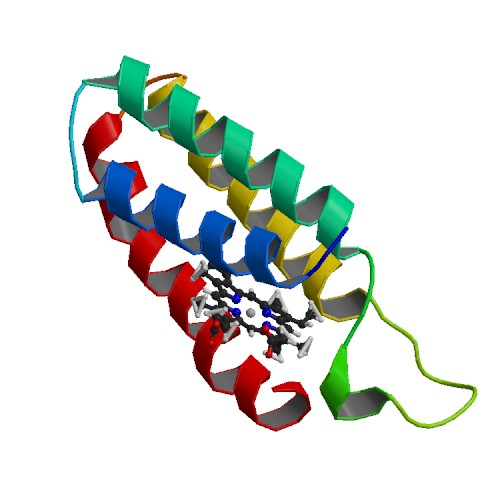
\includegraphics[width=30mm, trim= -10 -5 -5 -10]{1QPU_asym_r_500.jpg} & Topologie: \newline \textit{Four Helix Bundle} \newline Superfamilie: CATH: 1.20.120.10 & Der Eintrag beschreibt die Struktur des oxidierten Cytochrom B562 aus \textit{E. coli} \cite{1qpu}. Es ist am Elektronentransport beteiligt. \\ \hline
1QQ3  & 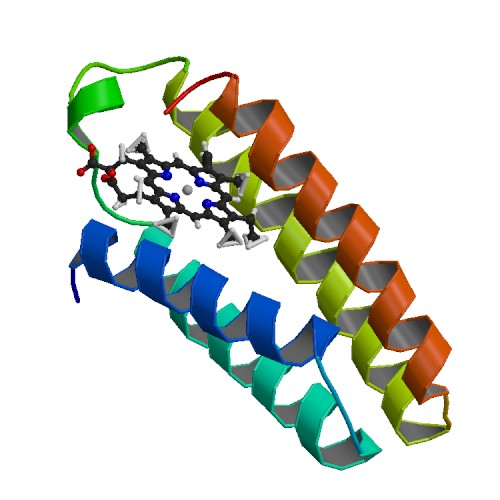
\includegraphics[width=30mm, trim= -10 -5 -5 -10]{1QQ3_asym_r_500.jpg} & Topologie: \newline \textit{Four Helix Bundle} \newline Superfamilie: CATH: 1.20.120.10  & Die Hem-bindende Variante des oxidierten Cytochrom B562 aus \textit{E. coli} wird durch diesen Eintrag beschrieben \cite{1qq3}. Auch diese Variante des Proteins ist f\"ur Elektronentransport zust\"andig. \\ \hline
1CGN  & 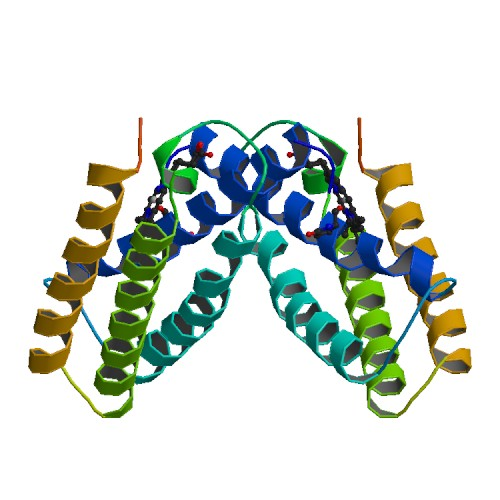
\includegraphics[width=30mm, trim= -10 -5 -5 -10]{1CGN_bio_r_500.jpg} & Topologie: \newline \textit{Four Helix Bundle} \newline Superfamilie: CATH: 1.20.120.10  & Dieser Eintrag beschreibt die Struktur von Cytochrom C' \cite{1cgn} aus \textit{Achromobacter xylosoxidans}. Es ist ebenfalls f\"ur Elektronentransport zust\"andig. \\ \hline
1HE9  & 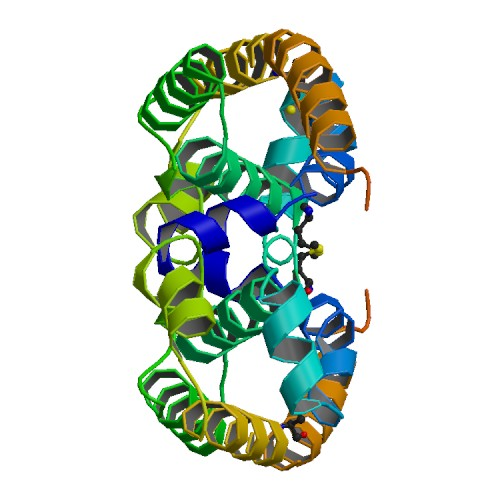
\includegraphics[width=30mm, trim= -10 -5 -5 -10]{1HE9_bio_r_500.jpg}  & Topologie: \newline \textit{Four Helix Bundle} \newline Superfamilie: \newline \textit{Bacterial GAP Domain}   & Der Eintrag beschreibt die GTPase aktivierende Dom\"ane des Toxins Exoenzyms S aus \textit{Pseudomonas aeruginosa} \cite{1he9}. \\ \hline
3GF9  & 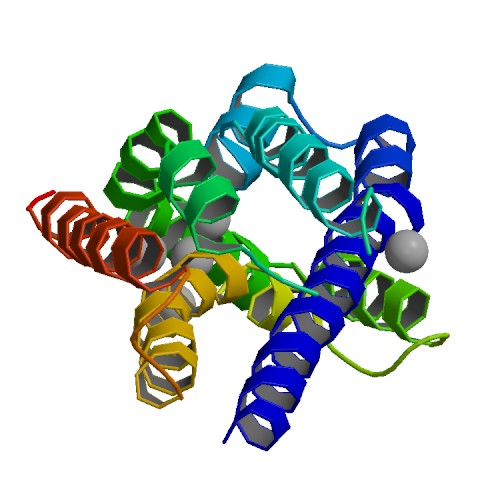
\includegraphics[width=30mm, trim= -10 -5 -5 -10]{3GF9_bio_r_500.jpg} & Topologie: \newline \textit{Dbl homology Domain} \newline Superfamilie: \newline DBL Homology Domain & Die RhoGEF-Dom\"ane des  Proteins Intersectin 2 aus \textit{Homo sapiens} wird durch den Eintrag 3GF9 beschrieben \cite{3gf9}. Dieses Protein ist f\"ur Endocytose zust\"andig. \\ 
\hline
\label{tab:occ_alpha}
\end{tabular}
\end{center}

\end{table}


\begin{table}
\begin{center}
\caption{Diese Tabelle zeigt die Strukturen der $\beta$-Proteine der Fallstudie. Alle Proteine in dieser Tabelle geh\"oren zur Architektur der $\beta$-\textit{Barrels}. Die Bilder der 3D-Strukturen und die Beschreibunng der Eintr\"age stammen aus der PDBund aus UniProt. Die Einordnung der Topologie und der Superfamilie stammt aus CATH. }
\begin{tabular}{ | C{9mm} | C{30mm} | C{29mm} | C{38mm} | }
\hline
PDB-ID & 3D Bild & Struktur & Beschreibung \\ \hline
1EXS  & 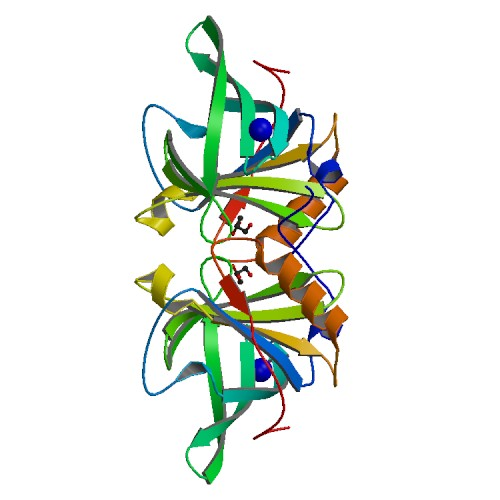
\includegraphics[width=30mm, trim= -10 -5 -5 -10]{1EXS_bio_r_500.jpg} & Topologie: \newline \textit{Lipocalin} \newline Superfamilie: CATH: 2.40.128.20 & Der Eintrag 1EXS beschreibt die Struktur des $\beta$-Lactoglobulin aus \textit{Sus scrofa} \cite{1exs}. Es ist ein lipidbindendes Protein. \\ \hline
1NGL  & 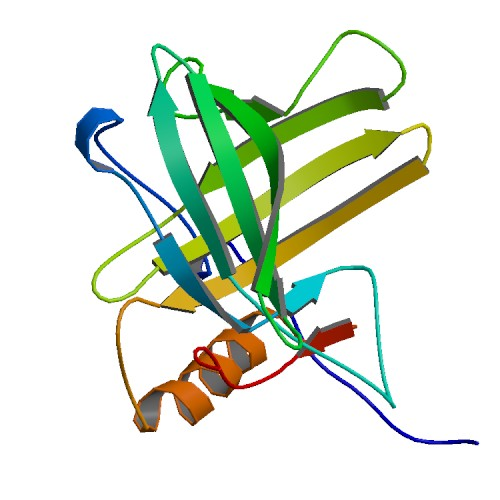
\includegraphics[width=30mm, trim= -10 -5 -5 -10]{1NGL_asym_r_500.jpg} & Topologie: \newline \textit{Lipocalin} \newline Superfamilie: CATH: 2.40.128.20  & Das neutrophile Gelatinase asoziierte Lipocalin des \textit{Homo sapiens} wird durch den Eintrag 1NGL beschrieben \cite{1ngl}. Es ist ein Transportprotein. \\ \hline
1QQS  & 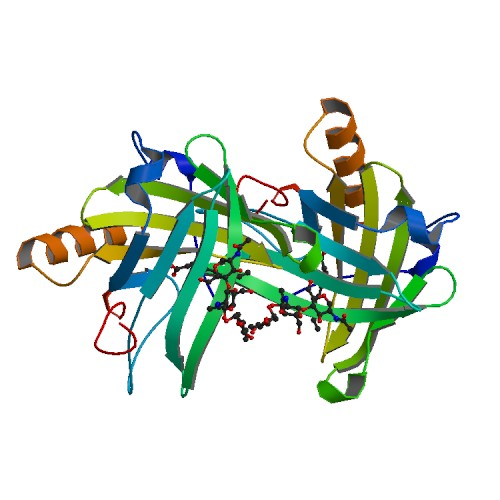
\includegraphics[width=30mm, trim= -10 -5 -5 -10]{1QQS_bio_r_500.jpg} & Topologie: \newline \textit{Lipocalin} \newline Superfamilie: CATH: 2.40.128.20  & Die Struktur des neutrophilen Gelatinase assoziierten Lipocalin Homodimers wird durch den Eintrag 1QQS beschrieben \cite{1qqs}. Es ist ein zuckerbindendes Protein.  \\ \hline
3SLO  & 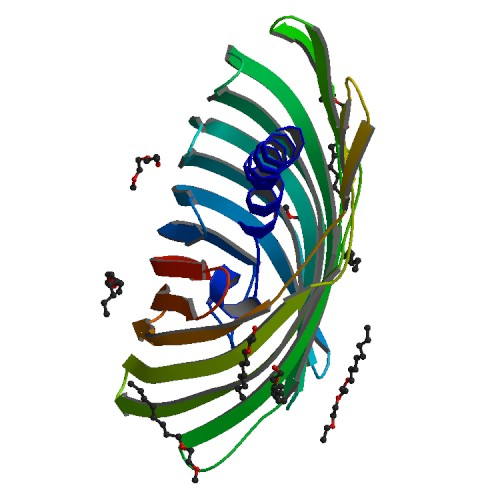
\includegraphics[width=30mm, trim= -10 -5 -5 -10]{3SLO_bio_r_500.jpg}  & Topologie: \newline \textit{Lipocalin} \newline Superfamilie: \newline Autortransporter Esterase   & Der Eintrag 3SLO beschreibt die Struktur der N1023D Mutante des Autotransporters EspP \cite{3slo} aus \textit{E. coli}. Dieses Protein ist f\"ur den Transport von Proteinen zust\"andig. \\ \hline
1WJX  & 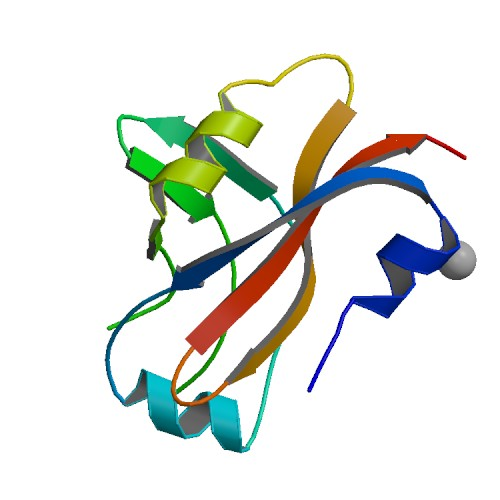
\includegraphics[width=30mm, trim= -10 -5 -5 -10]{1WJX_bio_r_500.jpg} & Topologie: \newline \textit{Small Protein B} \newline Superfamilie: \newline 2.40.280.10 & Dieser Eintrag beschreibt das Protein TT0801 aus \textit{Thermus thermophilus} \cite{1wjx}. \\ 
\hline

\label{tab:occ_beta}
\end{tabular}
\end{center}
\end{table}




\begin{table}
\begin{center}
\caption{Hier werden die $\alpha/\beta$-Proteine der Fallstudie gezeigt. Alle hier dargestellten Proteine haben eine \textit{3-Layer-Sandwich}-Architektur. Die Bilder und Beschreibungen entstammen UniProt und der PDB. Die Beschreibung der Struktur stammt aus CATH.}
\begin{tabular}{ | C{9mm} | C{30mm} | C{29mm} | C{38mm} | }
\hline
PDB-ID & 3D Bild & Struktur & Beschreibung \\ \hline
5CHY  & 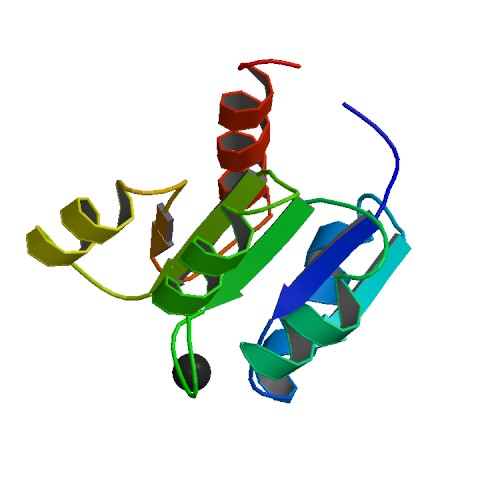
\includegraphics[width=30mm, trim= -10 -5 -5 -10]{5CHY_bio_r_500.jpg} & Topologie: \newline \textit{\textit{Rossman Fold}} \newline Superfamilie: CATH: 3.40.50.2300 & Der Eintrag beschreibt die Struktur einer Mutante des Chemotaxisproteins des Gens \textit{cheY} aus \textit{E. coli} \cite{5chy}. Es ist ein Signaltransduktionsproteinprotein. \\ \hline
2ID9  & 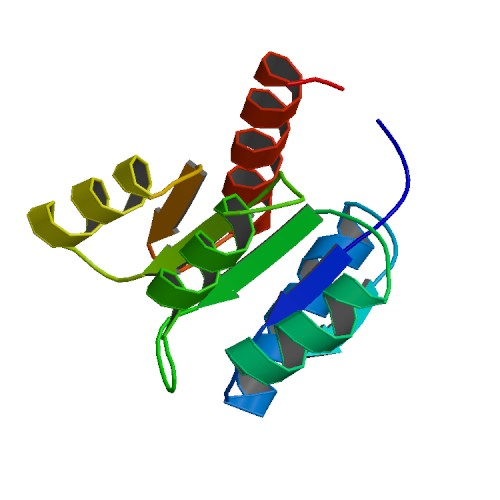
\includegraphics[width=30mm, trim= -10 -5 -5 -10]{2ID9_bio_r_500.jpg} & Topologie: \newline \textit{\textit{Rossman Fold}} \newline Superfamilie: CATH: 3.40.50.2300  & Der Eintrag beschreibt das synthetische Protein T87I phosphono-CheY \cite{2id9}. Es ist ein stabiles Analogon zu dem oben beschriebenen Chemotaxisprotein. \\ \hline
3I42  & 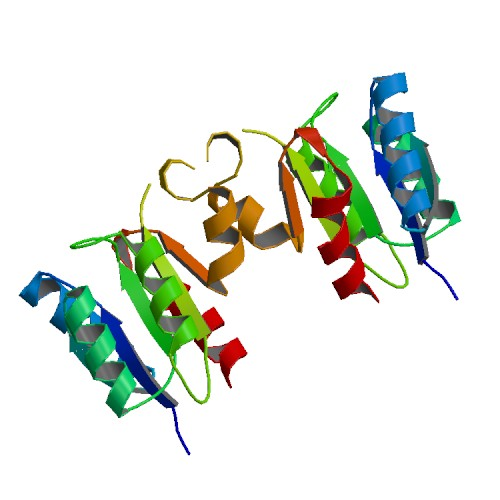
\includegraphics[width=30mm, trim= -10 -5 -5 -10]{3I42_bio_r_500.jpg} & Topologie: \newline \textit{\textit{Rossman Fold}} \newline Superfamilie: CATH: 3.40.50.2300  & Der Eintrag beschreibt eine Empfängerdom\"ane aus \textit{Methylobacillus flagellatus}, die regulatorische Signale empf\"angt und \"ahnlich zu \textit{cheY} ist \cite{3i42}.  \\ \hline
1D4O  & 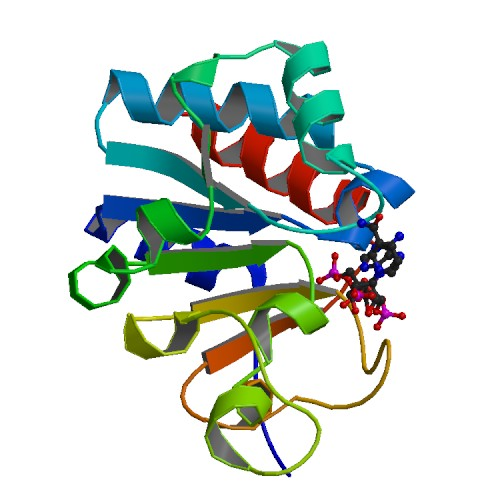
\includegraphics[width=30mm, trim= -10 -5 -5 -10]{1D4O_bio_r_500.jpg}  & Topologie: \newline \textit{Rossman Fold} \newline Superfamilie: \newline \textit{TPP-binding domain} & Die Struktur der Transhydrogenase Dom\"ane II aus \textit{Bos taurus} \cite{1d4o} wird durch diesen Eintrag beschreiben. Sie wird in der PDB als Oxidoreductase klassifiziert. \\ \hline
2W0I  & 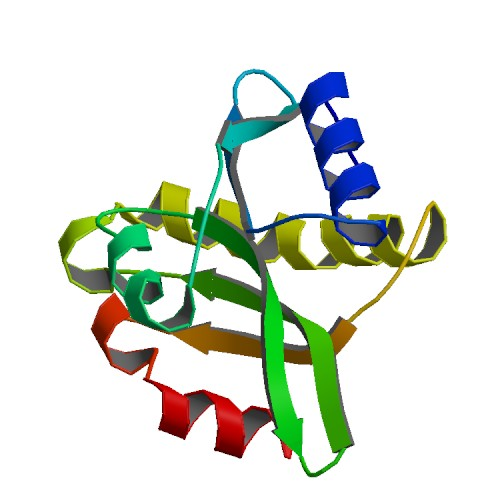
\includegraphics[width=30mm, trim= -10 -5 -5 -10]{2W0I_bio_r_500.jpg} & Topologie: \newline Severin \newline Superfamilie: \newline Severin & Der Eintrag beschreibt eine Dom\"ane des Proteins TWINFLIN-2 aus \textit{Homo sapiens} \cite{2woi}. Dieses Protein inhibiert die Polymerisation von Actin. \\ 
\hline

\label{tab:occ_ab}
\end{tabular}
\end{center}

\end{table}

F\"ur diesen Datensatz wurden alle \textit{Graphlet}-Vektoren berechnet. Die paarweisen Distanzen dieser Vektoren wurden mit der RGF und dem modifizierten Jaccard-Index berechnet. F\"ur die berechneten Distanzmatrizen wurden die Korrelationen der Distanzen in den verschiedenen Formaten berechnet und sie wurden mit den von PDBeFold berechneten Distanzen verglichen. 



\subsection{Der PDBTop500-Datensatz}

Der PDBTop500-Datensatz wurde von \textit{Lovell et al.} vorgestellt (\cite{top500}). Diese nutzten ihn zur Validierung von PDB-Strukturvorhersagen unter Verwendung der $\alpha$-C-Geometrie.
Der Datensatz enth\"alt 500 nicht redundante PDB-Eintr\"age mit einer Aufl\"osung von 1,8\AA{}  oder besser.

Er wurde ausgew\"ahlt, weil die \textit{Graphlet}-Vektoren f\"ur ihn schnell berechenbar waren. Im Gegensatz zu anderen Datens\"atzen mit nicht redundanten PDB-Eintr\"agen wie dem FATCAT- oder dem ASTRAL-Datensatz enth\"alt dieser keine riesigen Proteinkomplexe, deren \textit{Graphlets} auf durchschnittlichen Computern nicht in weniger als 24 Stunden berechnbar sind. 
Er ist aber immer noch gro"s genug, um Strukturvergleichsmethoden validieren zu k\"onnen. \textit{Zhang} und \textit{Skolnick} verwendeten zur Validierung von \textit{TM-align} einen Datensatz aus 200 PDB-Eintr\"agen (\cite{zhangtm}).

Da ein Vergleich der paarweisen Distanzen auf einem solchen Datensatz zu aufw\"andig war, wurde dieser Datensatz f\"ur eine statistische Analyse der \textit{Graphlet}-Vektoren genutzt.

F\"ur die relativen H\"aufigkeiten der einzelnen \textit{Graphlets} wurden Minima, Maxima, Varianzen und Durchschnittswerte berechnet. Hierbei war das Ziel festzustellen, ob wirklich alle \textit{Graphlets} f\"ur Strukturvergleiche notwendig sind.

Weiterhin wurde ein Datensatz aus Aldolasen zusammengestellt, um festzustellen, ob sich die Verteilungen der \textit{Graphlet}-H\"aufigkeiten, zwischen dem gro"sen Datensatz und den Aldolasen unterscheiden. Wenn der Unterschied der Verteilungen zwischen diesen beiden Datens\"atzen so gro"s ist, dass eine klare Unterscheidung m\"oglich ist, dann sollte auch eine maschinelle Klassifizierung der \textit{Graphlets} f\"ur Aldolasen m\"oglich sein. Aldolasen wurden gew\"ahlt, weil diese Superfamilie strukturell besonders divers ist \cite{das2015diversity}. Dabei betr\"agt die Sequenzidentit\"at der Proteine dieser Klasse immer mindestens 35\%.

Wenn die \textit{Graphlet}-Verteilungen der Aldolasen und des PDBTop500-Datensatzes klar unterscheidbar sind, dann sollten sie auch f\"ur Superfamilien, die strukturell einheitlicher sind unterscheidbar sein.

Die Aldolasen, die hier betrachtet sind in den Tabellen \ref{tab:aldolasen1} und \ref{tab:aldolasen2} aufgef\"uhrt.

\begin{table}
\begin{center}
\caption{Aldolasen Teil 1}
\begin{tabular}{ | C{9mm} | C{30mm} | C{29mm} | C{38mm} | }
\hline
PDB-ID & 3D Bild & Struktur & Beschreibung \\ \hline
1LBM  & 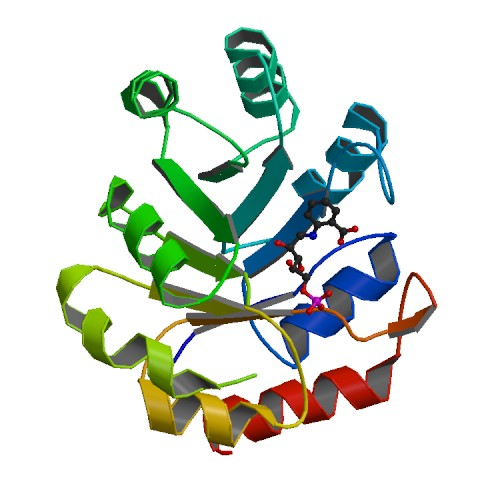
\includegraphics[width=30mm, trim= -10 -5 -5 -10]{1LBM_bio_r_500.jpg} & Topologie: \newline TIM \textit{Barrel} \newline Superfamilie: Aldolasen - Klasse I & Der Eintrag beschreibt die Phosphoribosyl Anthranilat Isomerase im Komplex mit einem Liganden aus \textit{Thermotoga maritima} \cite{1lbm}. Das Protein ist Teil des Stoffewechselweges zur Synthese von L-Tryptophan. \\ \hline
1LOR  & 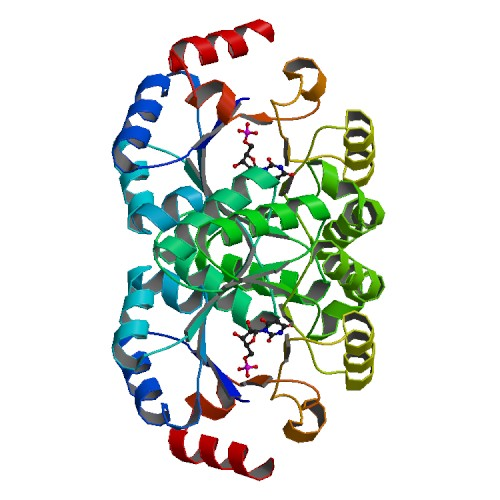
\includegraphics[width=30mm, trim= -10 -5 -5 -10]{1LOR_bio_r_500.jpg} & Topologie: \newline \textit{\textit{Rossman Fold}} \newline Superfamilie: CATH: 3.40.50.2300  & Die Struktur der Orotidin 5'-Monophosphatase aus \textit{Methanothermobacter thermautotrophicus} im Komplex mit einem Liganden wird durch diesen Eintrag beschrieben \cite{1lor}. Das Protein ist an der Decarboxylierung von Oritidin beteiligt. \\ \hline
1MXS  & 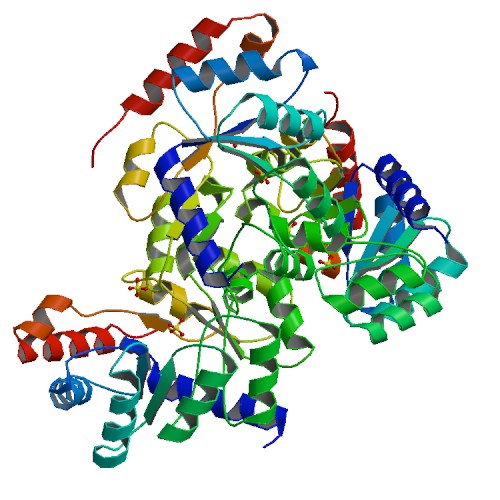
\includegraphics[width=30mm, trim= -10 -5 -5 -10]{1MXS_bio_r_500.jpg} & Topologie: \newline \textit{\textit{Rossman Fold}} \newline Superfamilie: CATH: 3.40.50.2300  & Dieser Eintrag beschreibt die 2-Keto-3-deoxy-6-Phosphogluconat Aldolase aus \textit{Pseudomonas putida} \cite{1mxs}. Genau wie die obigen Proteine wird dieses durch die PDB als Lyase klassifiziert. \\ \hline
1NSJ  & 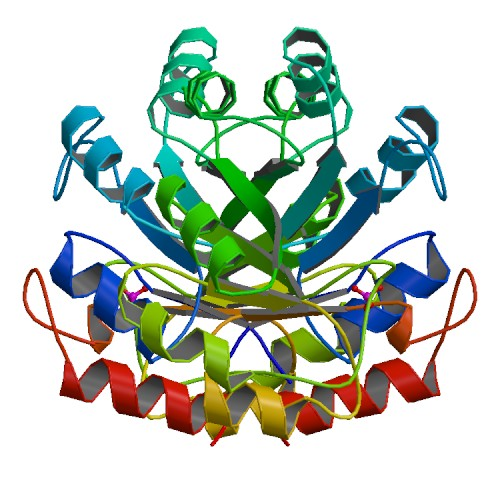
\includegraphics[width=30mm, trim= -10 -5 -5 -10]{1NSJ_bio_r_500.jpg}  & Topologie: \newline \textit{Rossman Fold} \newline Superfamilie: \newline \textit{TPP-binding domain} & Die Struktur der phosphoribosyl Anthranilat Isomerase aus \textit{Thermotoga maritima} wird duch diesen Eintrag beschrieben \cite{1nsj}. Auch dieses Protein ist in die Synthese von L-Tryptophan eingebunden. \\ \hline
1V5X  & 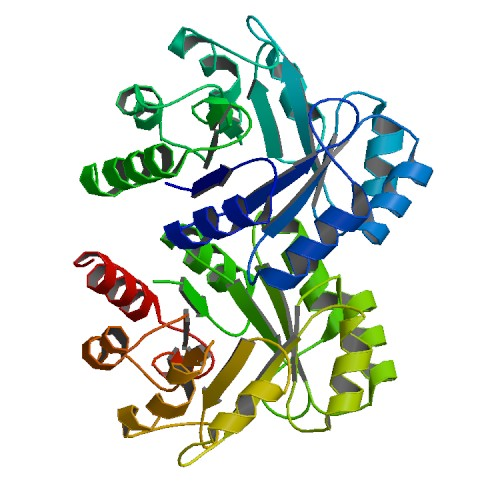
\includegraphics[width=30mm, trim= -10 -5 -5 -10]{1V5X_bio_r_500.jpg} & Topologie: \newline Severin \newline Superfamilie: \newline Severin & Auch dieser Eintrag beschreibt die Struktur einer Phosphoribosyl Anthranilat Isomerase \cite{1v5x}. Hier stammt sie aus \textit{Thermus thermophilus} und ist ebenfalls in die Synthese von L-Tryptophan eingebunden. \\ 
\hline

\label{tab:aldolasen1}
\end{tabular}
\end{center}
\end{table}

\begin{table}
\begin{center}
\caption{Aldolasen Teil II}
\begin{tabular}{ | C{9mm} | C{30mm} | C{29mm} | C{38mm} | }
\hline
PDB-ID & 3D Bild & Struktur & Beschreibung \\ \hline
1VQT  & 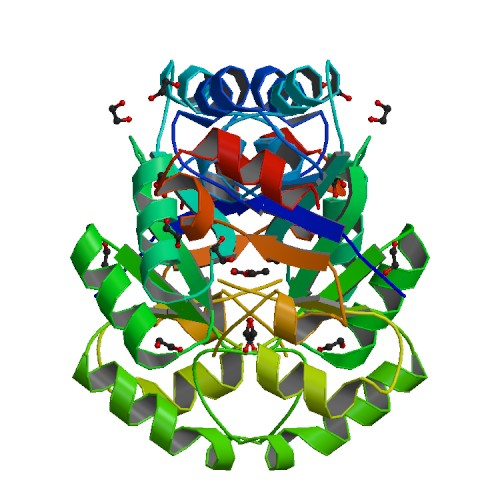
\includegraphics[width=30mm, trim= -10 -5 -5 -10]{1VQT_bio_r_500.jpg} & Topologie: \newline TIM \textit{Barrel} \newline Superfamilie: Aldolasen - Klasse I & Dieser Eintrag beschreibt die Struktur der Oritidin 5'-Phosphatase Decarboxylase aus \textit{Thermotoga maritima} \cite{1vqt}. Sie ist in die Synthese von UMP eingebunden. \\ \hline
1WAU  & 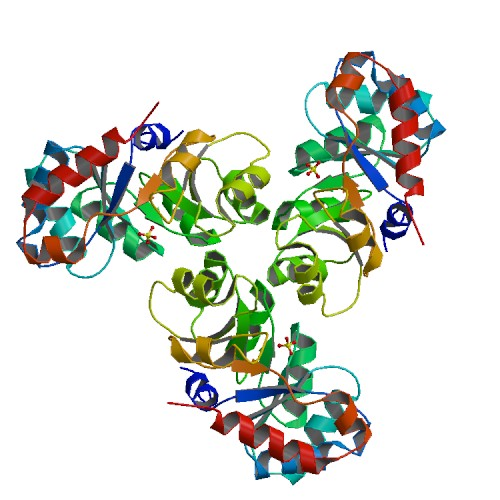
\includegraphics[width=30mm, trim= -10 -5 -5 -10]{1WAU_bio_r_500.jpg} &Topologie: \newline TIM \textit{Barrel} \newline Superfamilie: Aldolasen - Klasse I  & Der Eintrag beschreibt das synthetische Protein T87I phosphono-CheY \cite{2id9}. Es ist ein stabiles Analogon zu dem oben beschriebenen Chemotaxisprotein. \\ \hline
3CEU  & 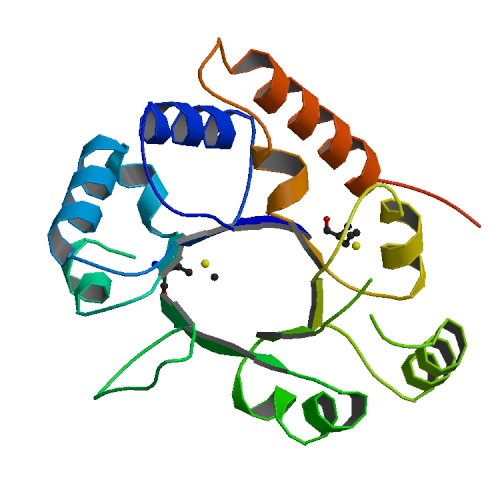
\includegraphics[width=30mm, trim= -10 -5 -5 -10]{3CEU_bio_r_500.jpg}  & Topologie: \newline TIM \textit{Barrel} \newline Superfamilie: Aldolasen - Klasse I & Hier wird die Struktur der E45N Mutante der KDPG-Aldolase aus \textit{E. coli} beschrieben \cite{3ceu}. Das Protein ist in den Glyoxylat und Dicarboxylat Stoffwechsel eingebunden. \\ \hline
7TIM  & 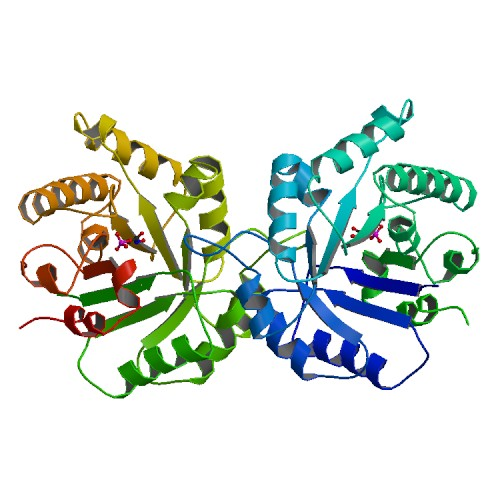
\includegraphics[width=30mm, trim= -10 -5 -5 -10]{7TIM_bio_r_500.jpg} & Topologie: \newline TIM \textit{Barrel} \newline Superfamilie: Aldolasen - Klasse I & Dieser Eintrag beschreibt einen Komplex aus der Triosephosphat Isoermase und Phophoglycolhydroxamat \cite{7tim}. Das Protein ist in die Gluconeogenese eingebunden.\\ 
\hline

% Abkuerzung: KDPG : 2-Keto-3-deoxy-phosphogluconate aldolase
\label{tab:aldolasen2}
\end{tabular}
\end{center}
\end{table}



\chapter{Ergebnisse}

\section{Der modifizierte Jaccard-Index}


Der Jaccard-Index ist ein Ma"s, um die \"Ahnlichkeit von gleichm\"achtigen Mengen zu bewerten. F\"ur zwei Mengen $A,B$ berechnet sich der Jaccard-Index $D_{Jac}(A,B)$ folgenderma"sen:

\[ D_{Jac}(A,B) := \frac{\sum_{x \ in A \land x \in B} 1}{\sum_{x \in A \lor x \in B} 1} \]

Dementsprechend sind zwei Mengen $A,B$ gleich, wenn  gilt $D_{Jac} = 1$ und disjunkt, wenn gilt $D_{Jac} = 0$. Mit ihm wird die relative Anzahl der Elemente beider Mengen berechnet.
Um dieses Ma"s in sinnvoller Weise auf \textit{Graphlet}-Vektoren zu \"ubertragen wurde ein zus\"atzlicher Faktor $k \in \mathbb{R} $ mit $k \in [0,1]$  eingef\"uhrt, der als Pr\"azisionsfaktor zu verstehen ist. Die Defintion des modifizierten Jaccard-Index $D_{JacM}(v,w)$ f\"ur zwei Vektoren $v,w$ lautet also:

\[ D_{JacM}(v,w) := \frac{\sum_{i = 1}^n x_i}{\sum_{x \in A \lor x \in B} 1} \]

Hierbei gilt:

\[ x_i = 
   \begin{cases}
     1     & \quad \mathrm{if} \quad v_i \geq w_i \times k \land w_i \geq v_i \times k \\
     0     & \quad \mathrm{else} \\
   \end{cases}
\]

In dieser modifizierten Variante werden zwei Vektoren $v,w$ als gleich angesehen, wenn sich $v_i,w_i$ f\"ur alle $i$ h\"ochstens um den Faktor $k$ unterschieden.
Dies steht im Gegensatz zur RGF, die -- analog zum euklidischen Abstand -- die Abst\"ande zwischen zwei \textit{Graphlet}-Vektoren misst.
F\"ur alle weiteren Messungen in dieser Arbeit wurde $k=0,9$ gew\"ahlt. Dies hatte den Grund, dass weder niedrigere noch h\"ohere Werte zu sinnvoller interpretierbaren Ergebnissen f\"uhrten.

\section{Der \textit{Graphlet}-Worte-Algorithmus}

In der letzten Version von \texttt{graphletAnalyser} war es bereits m\"oglich markierte \textit{Graphlets} mit 2 und 3 Knoten in Proteingraphen zu z\"ahlen. Diese Funktionalit\"at wurde im Rahmen dieser Arbeit verallgemeinert, so dass der Nutzer beliebige Alphabete angeben kann.
Der Algorithmus erh\"alt das Alphabet $\sum = \{ \sigma_i : i \in \mathbb{N} \}$ der Knotenmarkierungen. Aus diesem Alphabet berechnet er Worte $w$, die zur Repr\"asentation der markierten \textit{Graphlets} genutzt werden.
Hierbei k\"onnen verschiedene Worte das gleiche \textit{Graphlet} repr\"asentieren. Im Falle von 2-\textit{Graphlets} repr\"asentieren die zwei Worte $(\sigma_i,\sigma_j)$ und $(\sigma_j, \sigma_i)$ das gleiche markierte \textit{Graphlet} mit den Knotenmarkierungen $\sigma_i,\sigma_j$. Worte, die das gleiche \textit{Graphlet} repr\"asentieren, werden im Folgenden als \emph{\"aquivalente Graphlet-Worte}  bezeichnet.


Die Berechnung der \"aquivalenten \textit{Graphlet}-Worte der L\"ange 2 ist trivial. Aus dem Alphabet $\sum$ werden alle Worte $w = (\sigma_i, \sigma_j)$ berechnet, wobei Spiegelungen nicht mit ausgegeben werden, da zwei Worte $ (\sigma_j, \sigma_i) $ und $ (\sigma_j, \sigma_i) $ \"aquivalente \textit{Graphlet}-Worte sind.

Die Berechnung aller \"aquivalenten \textit{Graphlet}-Worte der L\"ange 3 ist komplizierter, da sie f\"ur zwei verschiedene \textit{Graphlets} berechnet werden m\"ussen. F\"ur das \textit{Graphlet} $g_1$ sind alle Worte \"aquivalent zueinander, die zyklische Vertauschungen voneinander sind. F\"ur das \textit{Graphlet} $g_2$ sind Worte \"aquivalent zueinander, die Spiegelungen voneinander sind (siehe Abbildung \ref{fig:3graphlets}). \\




\IncMargin{1em}
\begin{algorithm}
\SetKwData{Left}{left}\SetKwData{This}{this}\SetKwData{Up}{up}
\SetKwFunction{Union}{Union}\SetKwFunction{FindCompress}{FindCompress}
\SetKwFunction{add}{add}
\SetKwInOut{Input}{input}\SetKwInOut{Output}{output}
\Input{Ein Alphabet $ \sum = \{ \sigma_1, ... , \sigma_n \}$ }
\Output{Zwei Listen Wortliste-3-Weg, Wortliste-3-Kreis, die die repr\"asentierenden Worte f\"ur den Kreis bzw. Weg aus 3 Knoten beschreiben}
\BlankLine
\For{$i\leftarrow 1$ \KwTo $n$}{
Wortliste-3-Weg.\add{$\sigma_i \sigma_i \sigma_i$} \\
Wortliste-3-Weg.\add{$\sigma_i \sigma_i \sigma_i$} \\
\For{$k\leftarrow i+1$ \KwTo $n$}{


Wortliste-3-Weg.\add{$\sigma_i \sigma_k \sigma_i$} \\
Wortliste-3-Weg.\add{$\sigma_i \sigma_i \sigma_k$} \\
Wortliste-3-Weg.\add{$\sigma_i \sigma_k \sigma_k$} \\
Wortliste-3-Weg.\add{$\sigma_k \sigma_i \sigma_k$} \\

Wortliste-3-Kreis.\add{$\sigma_i \sigma_k \sigma_i$} \\
Wortliste-3-Kreis.\add{$\sigma_i \sigma_k \sigma_k$} \\

\For{$ m \leftarrow k + 1 $ \KwTo $n$}{
Wortliste-3-Weg.\add{$\sigma_i \sigma_k \sigma_m$} \\
Wortliste-3-Weg.\add{$\sigma_m \sigma_i \sigma_k$} \\
Wortliste-3-Weg.\add{$\sigma_k \sigma_m \sigma_i$} \\
Wortliste-3-Kreis.\add{$\sigma_i \sigma_k \sigma_m$} \\
Wortliste-3-Kreis.\add{$\sigma_m \sigma_k \sigma_i$} \\
}
}
}
\caption{\textit{Graphlet}-Worte-Algorithmus}\label{algo_gwords}
\end{algorithm}\DecMargin{1em}


Der Algorithmus besteht aus drei \textit{for}-Schleifen, die \"uber das Alphabet iterieren. In der jeder dieser Schleifen werden alle \"aquivalenten Worte hinzugef\"ugt, die aus den aktuell betrachteten Buchstaben erzeugt werden k\"onnen.


F\"ur das Alphabet der Protein- und Komplexgraphen $ \sum_{SSE} := \{ H, E, L \} $ und das Alphabet der Aminos\"auregraphen $ \sum_{AA} := \{ h, p, c, ? \} $ gibt der oben beschriebene Algorithmus die folgenden Listen aus:


\begin{subequations}
\begin{align*}
p_2 :=       (HH, HE, HL, EE, EL, LL) \\
p_{3-Weg}   := (HHH, HEH, HHE, HEE, EHE, \\
                HEL, LHE, ELH, HLH, HHL, \\
                HLL, LHL, EEE, ELE, EEL, \\
                ELL, LEL, LLL) \\
p_{3-Kreis} := (HHH, HEH, HEE, HEL, LEH, \\
                HLH, HLL, EEE, ELE, ELL, LLL) \\
\end{align*}
\end{subequations}

Die Vektoren $a_2, a_{3-Weg}$ und $a_{3-Kreis}$ beschreiben die Worte f\"ur \textit{Graphlets} in AA-Graphen 

\begin{subequations}
\begin{align*}
a_2 :=         (hh, hp, hc, h?, pp, pc, p?, cc, c?, ??) \\ 
a_{3-Weg} :=   (hhh, hph, hhp, hpp, php, hpc, chp, pch, hp?, ?hp,\\
                p?h, hch, hhc, hcc, chc, hc?, ?hc ,c?h, h?h, hh?, \\
                h??, ?h?, ppp, pcp, ppc, pcc, cpc, pc?, ?pc, c?p, \\
                p?p, pp?, p??, ?p?, ccc, c?c, cc?, c??, ?c?, ???) \\
a_{3-Kreis} := (hhh, hph, hpp, hpc, cph, hp?, ?ph, hch, hcc, hc?, \\
                ?ch, h?h, h??, ppp, pcp, pcc, pc?, ?cp, p?p, p??, \\
                ccc, c?c, c??, ???)
\end{align*}
\end{subequations}

% a2 laenge 10
% a3weg laenge 40
% a3kreis laenge 24

Um die Korrektheit des Algorithmus zu \"uberpr\"ufen wurde die Ausgabe f\"ur Alphabete mit 3 und 4 Buchstaben h\"andisch \"uberpr\"uft.


\section{Erweiterung von \texttt{graphletAnalyser}}

\paragraph{Das Einlesen von Komplexgraphen und Aminos\"auregraphen}

ist implementiert worden. Die entsprechenden Alphabete sind im Programmcode vordefiniert und k\"onnen vom Nutzer \"uber Parameter ausgew\"ahlt werden oder in der Konfigurationsdatei festgelegt werden.

\paragraph{Nutzerdefinierte Knotenmarkierungen} k\"onnen nun in der Konfigurationsdatei angegeben werden. Der Nutzer kann ein Alphabet von Knotenmarkierungen und ein \textit{Label}, unter dem diese Knotenmarkierungen in den GML-Dateien gespeichert sind, angeben. F\"ur dieses Alphabet werden alle \"aquivalenten \textit{Graphlet}-Worte durch den \textit{Graphlet}-Worte-Algorithmus berechnet. Diese werden dann bei der Berechnung der markierten \textit{Graphlets} im Graphen unter dem vorgegebenen \textit{Label} gesucht und gez\"ahlt.
Es k\"onnen also beliebige Alphabete und \textit{Labels} angegeben werden, so lange die Markierungen der Knoten nicht mehr als einen Buchstaben enthalten.


 

\paragraph{Die Datenbankanbindung} wurde um Funktionen zum Speichern von Aminos\"auregraphen und Komplexgraphen erweitert. Das Speichern von Vektoren markierter \textit{Graphlets} wurde implementiert.

Wenn die Option \texttt{--useDatabase} ausgew\"ahlt wird, pr\"uft das Programm, ob der entsprechende Graph bereits in der Datenbank vorhanden ist. Falls der Graph gefunden wurde, wird der \textit{Graphlet}-Vektor f\"ur den entsprechenden Graphen in die Datenbank eingetragen. 



\section{Fallstudie}

Die paarweisen RGF-Distanzen der Proteine befinden sich in den Tabellen  \ref{table:occ-aag-rgf}, \ref{table:occ-pg-rgf} und \ref{table:occ-cg-tc}. Die paarweisen Jaccard-Indizes befinden sich in den Tabellen \ref{table:occ-aa-tc}, \ref{table:occ-pg-tf} und \ref{table:occ-cg-tc}.
Hierbei wurden die Zellen, die die 4 besten Bewertungen f\"ur das Protein der entsprechenden Zeile enthalten gr\"un eingef\"arbt. Das Gr\"un ist umso dunkler, je st\"arker die \"Ahnlichkeit bewertet wird.

\paragraph{Der Vergleich mittels RGF}
zeigt f\"ur die Aminos\"auregraphen die st\"arksten \"Ahnlichkeiten immer innerhalb der entsprechenden CATH-Klassen. Sowohl die Proteine aus der $\alpha$-Klasse als auch die Proteine der $\beta$-Klasse haben die besten \"Ahnlichkeitswerte mit Proteinen der gleichen Klasse.
Innerhalb der Klasse der $\alpha/\beta$-Proteine, gibt es mit 2id9 und 1d4o zwei Proteine, denen eine gr\"o"sere \"Ahnlichkeit zu Proteinen der \textit{mainly-alpha}-Klasse attestiert wurde.
Bei 1d4o f\"allt auf, dass der niedrigste Wert mit 7,091 deutlich h\"oher ist, als die besten Werte aller anderen Proteine.
2id9 hat laut der RGF-Distanz die gr\"o"ste \"Ahnlichkeit zu 1he9.
Bis auf diese beiden Au"snahmen l\"asst sich jedoch eine starke Korrelation mit den CATH-Klassen erkennen.
Alle anderen Proteine haben mindestens die zwei kleinsten RGF-Distanzen zu Vertretern aus der selben CATH- und SCOPe-Klasse.

Dies gilt f\"ur die Aminos\"auregraphen. Die RGF-Distanzen der Proteingraphen zueinander zeigen ein weniger klares Bild.
F\"ur die $\alpha$-Klasse und die der $\beta$-Klasse befinden sich die Proteine mit den k\"urzesten Distanzen immer noch in der selben Klasse. Dies l\"asst sich f\"ur die Proteine der $\alpha/\beta$-Klasse aber nicht mehr behaupten. Hier haben 2id9, 3i42 und 2w0i die k\"urzesten Distanzen zu Proteinen anderer Klassen.

Bei den Komplexgraphen ist die Korrelation zwischen der RGF-Distanz und der Zugeh\"origkeit zur strukturellen Klasse noch geringer. Die Tabelle \ref{table:occ-cg-rgf} zeigt nur f\"ur die Proteine 1qq3, 1he9, 1exs und 1qqs die k\"urzeste Distanz zu einem Vertreter der gleichen Klasse.
Es f\"allt jedoch auf, dass besonders h\"aufig die Proteine der \textit{alpha-beta}-Klasse 5chy, 2id9 und 3i42 als \"ahnlich zu anderen bewertet werden.

\paragraph{Der Vergleich der Jaccard-Indizes}
zeigt ein \"ahnliches Bild, wie der Vergleich der RGF-Distanzen. Bei den Aminos\"auregraphen zeigt sich, dass innerhalb der $\alpha$-Klasse wieder die paarweisen \"Ahnlichkeiten der $\alpha$-Proteine am gr\"o"sten sind. Dies gilt bis auf eine Ausnahme auch f\"ur die $\beta$-Proteine. Das Protein mit der PDB-ID 1ngl wird als strukturell \"ahnlichstes Protein zu 2w0i bewertet. In der Klasse der $\alpha/\beta$-Proteine gibt es mit 2ID9 und 1D4O wieder zwei Ausrei"ser, die die gr\"o"sten paarweisen \"Ahnlichkeiten nicht zu Vertretern der eigenen Klasse haben. F\"ur 2ID9 wird 1HE9 als \"ahnlichstes Protein angegeben und 1D4O wird 1QQS zugeordnet.

Die paarweisen modifizierten Jaccard-Indizes der Proteingraphen zeigen - wie schon bei den RGF-Distanzen - eine geringere Korrelation mit der Zugeh\"origkeit zu den CATH-Klassen, als die Koeffizienten der Aminos\"auregraphen. Es haben zwar wieder mindestens 3 Vertreter jeder Klasse ihren n\"achsten Nachbarn in der gleichen Klasse, aber es gibt auch einige Proteine, die ihren n\"achsten Nachbarn au"serhalb der eigenen Klasse haben. Hierzu geh\"oren 1d4o und 2w0i, die $\alpha/\beta$-Proteine sind, und das $\alpha$-Protein 3GF9. Es f\"allt auf, dass wieder die Proteine mit den PDB-DIs 2id9 und 3i42 besonders h\"aufig als strukturell \"ahnlich zu vielen anderen Proteinen bewertet werden.

F\"ur die Komplexgraphen zeigt die Tabelle wieder eine hohe \"Ahnlichkeite unter den ersten drei Proteinen 1qpu, 1qq3 und 1cgn. Auch innerhalb der Klasse $\alpha/\beta$ sind drei Proteine mit der h\"ochsten paarweisen \"Ahnlichkeit bewertet worden. Die geringe Anzahl von stark bewerteten \"Ahnlichkeiten innerhalb der $\beta$-Klasse ist sehr auff\"allig. 1qqs und 3slo sind das einzige Paar mit $\beta$-Topologie, dessen \"Ahnlichkeit als gro"s bewertet wurde.


\section{PDBTop500-Datensatz}

F\"ur den PDBTop500-Datensatz wurden \textit{Graphlet}-Vektoren der drei verschiedenen Graphenformate berechnet. Diese Vektoren wurden f\"ur jedes Format in einer .csv-Datei zusammengefasst und f\"ur jede dieser Dateien wurden \textit{Boxplots} erstellt.

In diese Boxplots wurden zus\"atzlich die relativen H\"aufigkeiten der bereits beschriebenen Aldolasen eingetragen. Hiermit kann festgestellt werden, ob die Superfamilie der Aldolasen anhand ihrer \textit{Graphlets} von anderen Superfamilien unterscheidbar ist.
Der Boxplot \ref{fig:aaplot} stellt diese Daten f\"ur die Aminos\"auregraphen dar. Da die relativen H\"aufigkeiten der \textit{Graphlets} in den Aminos\"auren deutlich kleiner sind als bei Proteingraphen und Komplexgraphen, weil es f\"ur sie mehr \textit{Graphlet}-Worte gibt, wurde die Skala der y-Achse logarithmiert.



\begin{sidewaysfigure}

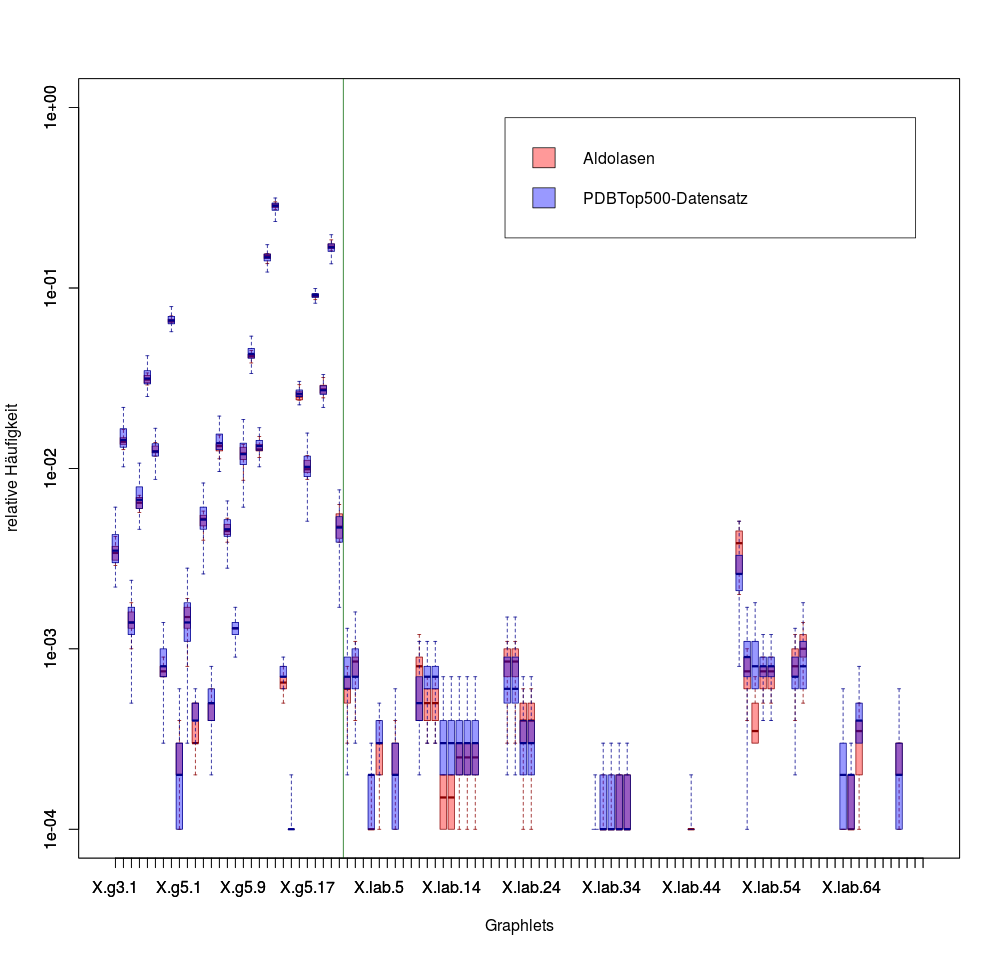
\includegraphics[scale=0.55]{aa_plot.png}
\caption{Verteilung der relativen H\"aufigkeiten der \textit{Graphlets} in Aminos\"auregraphen. Jeder Punkt auf der x-Achse entspricht einem \textit{Graphlet}. Die y-Achse ist logarithmiert und beschreibt die relative H\"aufigkeiten. Die H\"aufigkeiten der Proteine des PDBTop500-Datensatzes sind in blau, die der Aldolasen in rot angegeben. Links von der vertikalen Linie sind \textit{Graphlets} ohne Markierungen, rechts davon sind \textit{Graphlets} mit Markierungen. Ausrei"ser sind nicht eingetragen.}
\label{fig:aaplot}
\end{sidewaysfigure}




Unter den \textit{Graphlets} ohne Markierungen in Abbildung \ref{fig:aaplot} gibt es nur zwei bei denen sich die relativen H\"aufigkeiten der Aldolasen nicht mit denen des Datensatzes \"uberlappen. Dies sind die \textit{Graphlets} $g_8$ und $g_{15}$ in \ref{fig:5graphlets}, die in den Aldolasen nicht gefunden werden.


Unter den markierten \textit{Graphlets} gibt es deutlich mehr Unterschiede. Sieben verschiedene \textit{Graphlet}-Verteilungen \"uberlappen sich nicht. Die ersten drei hiervon entsprechen den \textit{Graphlet}-Worten h?, c? und ??. Diese stehen f\"ur Kanten zwischen unpolaren Residuen und Liganden, Kanten zwischen sauren oder basischen Residuen und Liganden und Kanten zwischen Liganden.

Die n\"achsten drei Worte f\"ur die keine \"Uberlappungen gefunden wurden sind die Worte hhh, hph und hhp. Diese repr\"asentieren Wege der L\"ange 2 zwischen drei unpolaren Residuen, zwei unpolaren Residuen mit einem polaren Residuum als inneren Knoten und zwei unpolaren Residuen mit einer polaren Aminos\"aure als Endknoten.


\begin{sidewaysfigure}

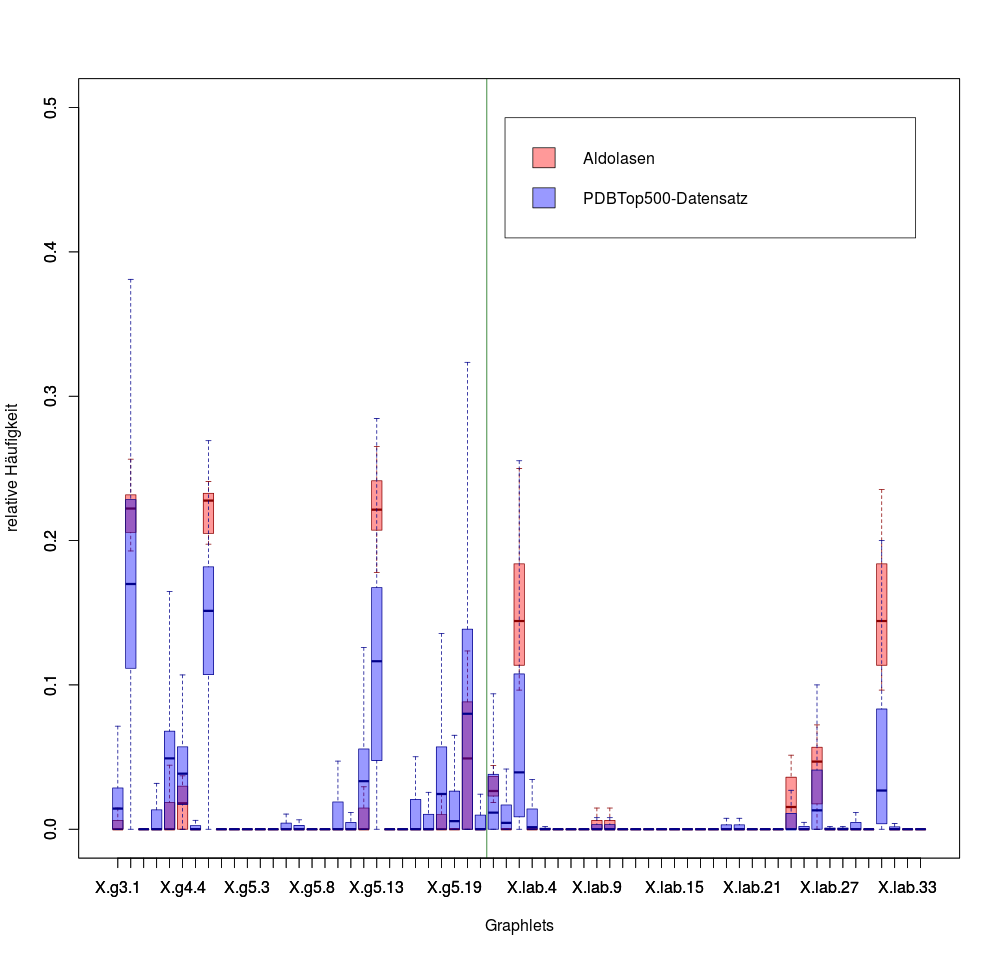
\includegraphics[scale=0.55]{pg_plot.png}
\caption{Verteilung der relative H\"aufigkeiten der \textit{Graphlets} f\"ur Proteingraphen. Auch hier entspricht jeder Punkt auf der x-Achse einem \textit{Graphlet} und die y-Achse zeigt die relativen H\"aufigkeiten an. Wieder trennt die dunkelgr\"une Linie markierte und nicht markierte \textit{Graphlets}. Solche ohne Markierungen sind links, mit Markierungen Versehene befinden sich rechts.}
\label{fig:pgplot}
\end{sidewaysfigure}

Bei den Proteingraphen in Abbildung \ref{fig:pgplot} sind die \textit{Graphlet}-Verteilungen ein wenig st\"arker voneinander getrennt.  
Dies gilt f\"ur das 4-\textit{Graphlet} $g_6$, das 5-\textit{Graphlet} $g_13$. Unter den markierten \textit{Graphlets} ist die Trennung f\"ur die am st\"arksten, die durch die Worte HL und HLL markiert werden. Ersteres repr\"asentiert den Kontakt einer $\alpha$-Helix mit einem Liganden. Letzteres markiert einen Kreis, in dem zwei Liganden mit einer Helix in Kontakt stehen.


\begin{sidewaysfigure}

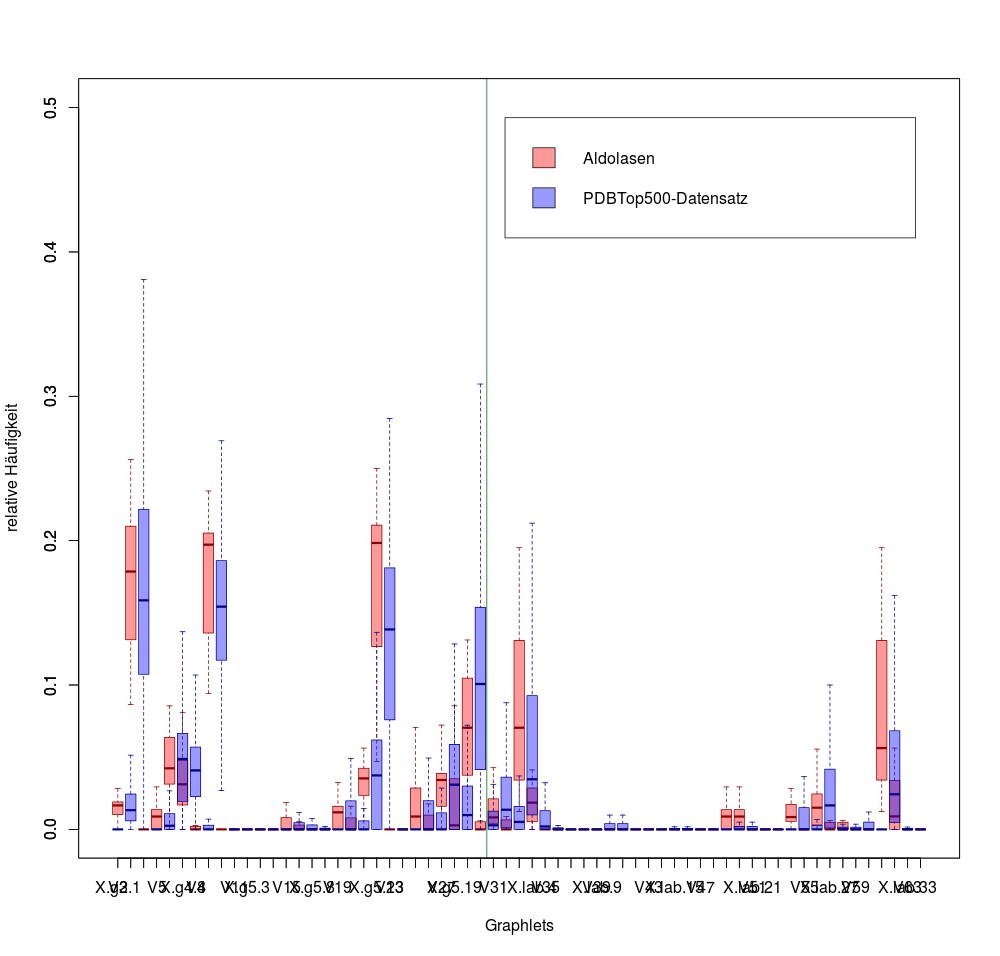
\includegraphics[scale=0.55]{cg_plot.png}
\caption{Verteilung der relative H\"aufigkeiten der \textit{Graphlets} f\"ur Komplexgraphen. Auch hier entspricht jeder Punkt auf der x-Achse einem \textit{Graphlet} und die y-Achse zeigt die relativen H\"aufigkeiten an. Wieder trennt die dunkelgr\"une Linie markierte und nicht markierte \textit{Graphlets}. Solche ohne Markierungen sind links, mit Markierungen versehene befinden sich rechts.}
\label{fig:cgplot}
\end{sidewaysfigure}

F\"ur die Komplexgraphen in Abbildung \ref{fig:cgplot} finden wir die st\"arksten Unterschiede zwischen den Verteilungen der Aldolasen und denen des Referenzdatensatzes. F\"ur die unmarkierten \textit{Graphlets} $g_1$ und $g_2$ in \ref{fig:3graphlets}, $g_2$, $g_3$ und $g_6$ in \ref{fig:4graphlets} sowie $g_6$, $g_{10}$, $g_{12}$, $g_{13}$, $g{16}$, $g_{18}$, $g_{20}$ und $g_{21}$ in \ref{fig:5graphlets}.
Die st\"arksten Abweichungen der Verteilungen finden wir bei den markierten \textit{Graphlets} f\"ur jene, die durch die Worte HL, LLL, und EEE repr\"asentiert sind. F\"ur das Wort LL finden wir diese Abweichungen sowohl f\"ur das markierte \textit{Graphlet}, das $g_1$ in \ref{fig:3graphlets} entspricht, als auch f\"ur jenes, das $g_2$ repr\"asentiert.
Damit sind die Unterschiede der \textit{Graphlet}-Verteilungen zwischen dem Referenzdatensatz und den Aldolasen in den Komplexgraphen am gr\"o"sten.


\chapter{Diskussion und Ausblick}




Die folgende Diskussion widmet sich vor allem der Frage, wieso die Ergebnisse der \"Ahnlichkeitsvergleiche sich so stark zwischen den jeweiligen Graphendarstellungen unterscheiden.
Des weiteren wird der Zusammenhang zwischen dem modifizierten Jaccard-Index und der RGF untersucht.

\section{Diskussion}

\subsection{Fallstudie}
\subsubsection{Vergleich der Graphtypen}

Wie schon im Ergebnisteil dargestellt, zeigen die Vergleiche der Aminos\"auregraphen den h\"ohsten Konsens mit der Einteilung der Strukturen durch CATH und SCOPe. Eine m\"ogliche Erkl\"arung hierf\"ur ist die Gestalt der Graphen. Bisher wurden \textit{Graphlets} zur Analyse von zusammenh\"angenden Graphen verwendet (\cite{sherv_graphlets}, \cite{graphletfrequency}).
Proteingraphen und Komplexgraphen sind jedoch nicht immer zusammenh\"angend. es kommt h\"aufig vor, dass einzelne Knoten keine Verbindungen zum Rest des Graphen aufweisen. Dies kommt daher, dass \textit{Coils} nicht modelliert werden. Das unten stehende Bild zeigt ein Beispiel.

\begin{figure}[h!]
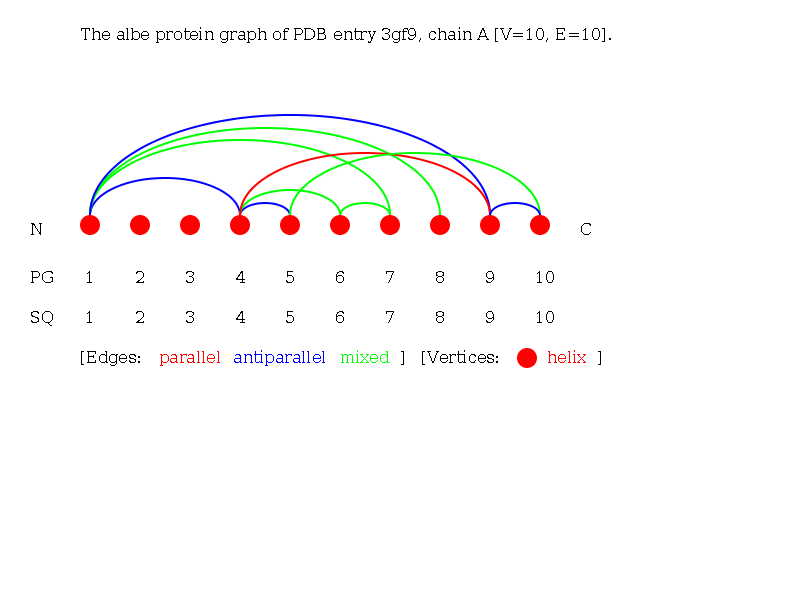
\includegraphics[scale=0.5]{3gf9_A_albe_PG.png}
\caption{Proteingraph von 3GF9 - Datensatz 1}
\end{figure}

Dadurch, dass dies in den zusammenh\"angenden \textit{Graphlets} nicht ber\"ucksichtigt werden kann, geht Information verloren. Unabh\"angig von der Wahl des \"Ahnlichkeitsma"s w\"urde dieser Graph mit einem anderen Graphen, dem die beiden Helix-Knoten mit einem Grad von 0 fehlen, als gleich bewertet werden, obwohl dieser zwei SSEs weniger aufwiese. Diese SSEs k\"onnen jedoch biologisch von zentraler Bedeutung sein.

Im Gegensatz hierzu sind die Aminos\"auregraphen dieser Fallstudie zusammenh\"angend, weil sie alle Residuen in der Polypeptidkette modellieren. Dies erkl\"art die h\"ohere Genauigkeit.


\subsubsection{Vergleich der Distanzma"se}

Wirft man einen Blick in die Tabellen, sieht es zun\"achst so aus, als w\"urden sich Jaccard-Index und RGF \"ahnlich gut eignen, um die \"Ahnlichkeit der \textit{Graphlet}-Vektoren zu bewerten. Die RGF stellt eine \emph{Distanz} zwischen zwei Vektoren dar. Dementsprechend steht ein RGF-Wert von 0 f\"ur die Gleichheit zweier Vektoren, je h\"oher der Wert ist, desto h\"oher ist der Abstand zwischen den beiden Vektoren. Der modifizierte Jaccard-Index, der hier Verwendung findet, z\"ahlt Elemente, die sich um h\"ochstens einen Faktor $k$ unterscheiden. Ein RGF-Wert von 1 bedeutete, dass alle Elemente beider Vektoren sich h\"ochstens um den Faktor $k$ unterscheiden. Ein Wert von 0 bedeutet, dass alle Elemente sich um mehr als den Faktor $k$ unterscheiden. Dementsprechend w\"urde man erwarten, dass die \textit{Pearson}-Korrelation von RGF und Jaccard-Index negativ ist. Die Tabelle \ref{tab:correlation} zeigt jedoch, dass diese f\"ur die Messungen der Fallstudie positiv ausf\"allt. 

\begin{table}
\begin{tabular}{ | c | c | }
\hline
Datensatz           & Korrelation \\ \hline
Aminos\"auregraphen &   0.6052    \\ \hline
Proteingraphen      &   0.3102    \\ \hline      
Komplexgraphen      &   0.1256    \\ \hline
\end{tabular}
\caption{Korrelationen der RGF mit den Jaccard-Indizes f\"ur die verschiedenen Graphtypen}
\label{tab:correlation}

\end{table}

Eine m\"ogliche Erkl\"arung hierf\"ur ist, dass die \textit{Graphlet}-H\"aufigkeiten bei der RGF logarithmiert werden, dadurch werden die gr\"o"sten Werte zu den kleinsten und andersrum.
So tragen Werte in \"ahnlichen Gr\"o"senordnungen immer zu einer k\"urzeren Distanz bei, obwohl sich die tats\"achlichen absoluten H\"aufigkeiten stark unterscheiden. Damit werden selten auftretende \textit{Graphlets} st\"arker f\"ur die Distanz gewichtet als solche, die h\"aufig auftreten. 



Beim Betrachten der relative n\textit{Graphlet}-H\"aufigkeiten haben wir gesehen, dass f\"ur die \textit{Graphlets}, die besonders h\"aufig sind, auch die Varianz dieser H\"aufigkeiten besonders gro"s ist, w\"ahrend gleichzeitig einige \textit{Graphlets} fast nie auftauchen.

Diese seltenen \textit{Graphlets} sorgen daf\"ur, dass der Jaccard-Index wahrscheinlich nie f\"ur ein Paar aus zwei beliebigen Proteinen den Wert Null annimmt. Damit wird bereits eine gewisse Mindest\"ahnlichkeit vorausgesetzt. Gleichzeitig ist kann der Jaccard-Index aber \textit{Graphlets}, die selten auftreten nicht st\"arker gewichten, denn wenn ein seltenes \textit{Graphlet} in einem Graphen einmal auftaucht und in einem anderen zweimal ist dieser Unterschied zu gro"s, um in eine positive Bewertung einzuflie"sen, obwohl dies eine starke \"Ahnlichkeit bedeuten k\"onnte.
Diese Form von \"Ahnlichkeit wird in der RGF ber\"ucksichtigt.

\subsubsection{Vergleich mit \textit{PDBeFold} - die Ausrei"ser}

Da \textit{PDBeFold} keine 15 Proteine auf einmal alignieren kann und ein \textit{Template}-basiertes Alignment durchf\"uhrt, wurde f\"ur den Vergleich mit den \textit{Graphlet}-Abst\"anden eine Teilmenge der Proteine ausgew\"ahlt.


Beim Vergleich der Komplexgraphen in Tabelle \ref{table:occ-cg-rgf} f\"allt auf, dass die Proteine 2id9, 3i42 und 2w0i die die geringsten Distanzen zu 1cgn haben, obwohl  1qq3 sein \"Ahnlichstes sein sollte. Ein multipler Vergleich dieser Proteine mit \textit{PDBeFold} ist in der Tabelle \ref{table:efold-comp1} zu sehen.



\begin{table}
\begin{tabular}{ | c | c | c | c | c | c | }
\hline
PDB & 1cgn    & 2id9  & 3i42  & 2w0i  & 1qq3 \\ \hline
1cgn &        & 1.357 & 1.497 & 3.554 & 1.757 \\ \hline
2id9 & 1.357  &       &       & 2.982 & 1.651 \\ \hline
3i42 &  1.497 & 0.405 &       & 3.066 & 1.866 \\ \hline
2w0i & 3.554  & 2.982 & 3.066 &       & 3.109  \\ \hline
1qq3 & 1.757  & 1.651 & 1.866 & 3.109 &       \\ \hline
\end{tabular}
\label{table:efold-comp1}
\caption{Alignmenttabelle aus  \textit{PDBeFold}. In den Zellen sind die \textit{Root-mean-square deviations} f\"ur die einzelnen Paare eingetragen.}
\end{table}


Sie zeigt, dass \textit{PDBeFold} die \"Ahnlichkeit des $\alpha$-Proteins 1cgn zu den $\alpha$/$\beta$-Proteinen 2id9 und 3i42 h\"oher bewertet, als die \"Ahnlichkeit zu dem $\alpha$-Protein 1qq3, obwohl diese in der gleichen Superfamilie einzuordnen sind. Somit stimmen die Bewertungen der \textit{Graphlet}-Vergleiche teilweise mit denen durch \textit{PDBeFold} \"uberein. Der einzige Unterschied in diesem Alignment ist, dass das Paar 1qq3, 1cgn als dritt\"ahnlichstes bewertet wurde, w\"ahrend es beim \textit{Graphlet}-Vergleich als viert\"ahnlichstes eingeordnet wurde.


Die starke \"Ahnlichkeit der $\beta$-Proteine zu den $\alpha$/$\beta$-Proteinen l\"asst sich erkl\"aren, wenn man die entsprechenden Graphen aus der PTGL betrachtet. Diese sind in den Abbildungen \ref{fig:2id9}, \ref{fig:3i42} und \ref{fig:2w0i} dargestellt:

\begin{figure}
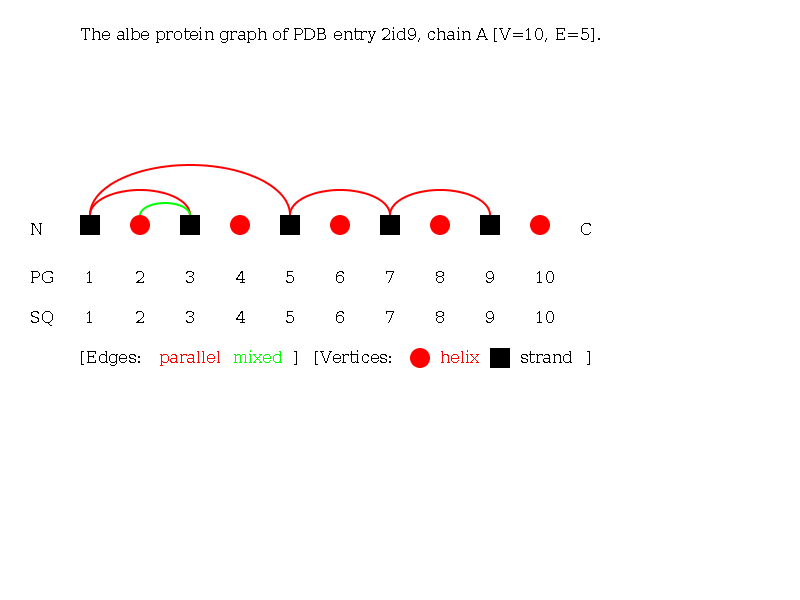
\includegraphics[scale=0.5]{2id9_A_albe_PG.png}
\label{fig:2id9}
\caption{Proteingraph von 2id9 \textit{Sch\"afer et al.}}
\end{figure}

\begin{figure}
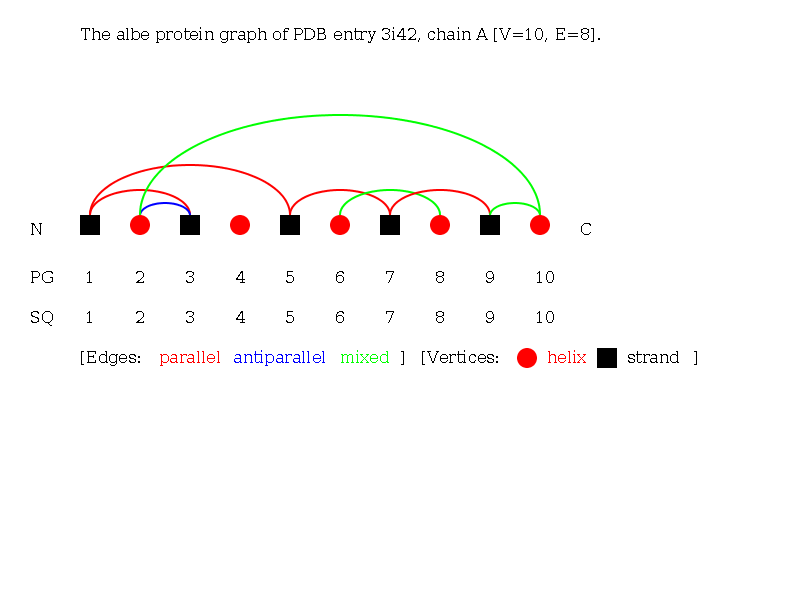
\includegraphics[scale=0.5]{3i42_A_albe_PG.png}
\label{fig:3i42}
\caption{Proteingraph von 3i42 \textit{Sch\"afer et al.}}
\end{figure}

\begin{figure}
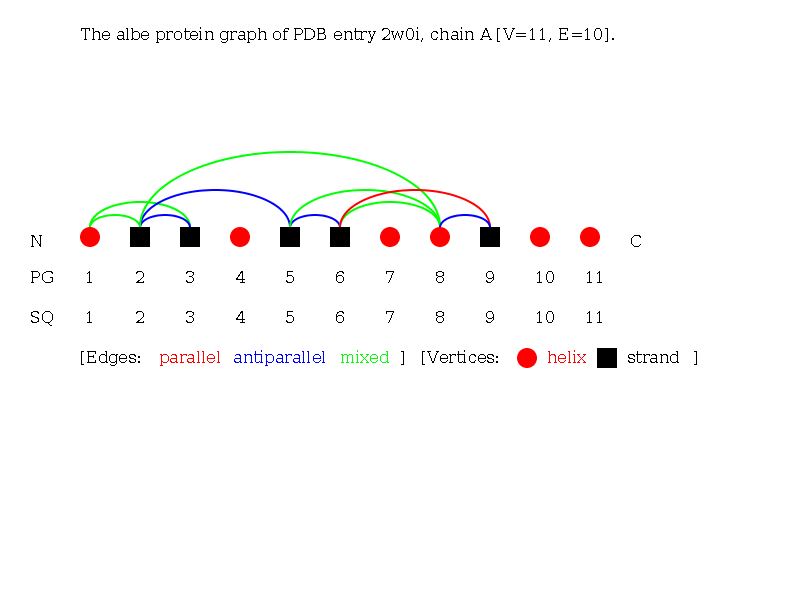
\includegraphics[scale=0.5]{2w0i_A_albe_PG.png}
\label{fig:2w0i}
\caption{Proteingraph von 2w0i \textit{Sch\"afer et al.}}
\end{figure}

In all diesen Graphen haben die meisten Knoten, die $\alpha$-Helices repr\"asentieren keine adjazenten Knoten.
Damit flie"sen f\"ur keinen dieser Graphen mehr als zwei $\alpha$-Helices in die \textit{Graphlet}-Vektoren ein. Stattdessen finden sich nur die zusammenh\"angenden Teilgraphen dieser Graphen in den \textit{Graphlet}-Vektoren wieder und diese Teilgraphen bestehen fast nur aus Knoten die $\beta$-Faltbl\"atter repr\"asentieren.


\subsection{PDBTop500-Datensatz und Aldolasen}

Der Vergleich der Proteine aus dem PDBTop500-Datensatz mit den Aldolasen hat gezeigt, dass sich die Verteilungen der \textit{Graphlets} f\"ur einige \textit{Graphlets} so stark unterscheiden, dass eine klare Unterscheidung der beiden anhand ihrer Verteilungen m\"oglich zu sein scheint.

Bei den Aminos\"auregraphen scheint diese Unterscheidung dabei am schlechtesten m\"oglich zu sein, da sich die Verteilungen f\"ur nicht-markierte \textit{Graphlets} durch die Abwesenheit der \textit{Graphlets} $g_8$ und $g_{15}$ in den Aldolasen unterscheiden. Es ist nicht klar, ob diese \textit{Graphlets} wirklich in den meisten anderen Proteinen vorkommen, oder diese Unterscheidung nur durch wegen der geringen Anzahl der Strukturen, die im Datensatz vertreten sind, zustande kommt.
Bei den markierten \textit{Graphlets} unterscheiden sich die Verteilungen am st\"arksten f\"ur jene, die die r\"aumliche N\"ahe von SSEs und Liganden bzw. Liganden untereinander repr\"asentieren.
Auch hier ist es fraglich, ob dieses Merkmal zur Unterscheidung von Aldolasen von allen anderen Superfamilien wirklich geeignet ist, oder ob Liganden in dem Datensatz unterrepr\"asentiert sind. 

Es ist interessant zu sehen, dass die Unterschiede in den \textit{Graphlet}-Verteilungen f\"ur Proteingraphen und Komplexgraphen am st\"arksten ist, obwohl diese im multiplen Vergleich der Fallstudie die geringeren Zusammenh\"ange mit der strukturellen Einteilung durch CATH zeigten. Die Ursache hierf\"ur k\"onnen die verwendeten Metriken sein. Die hohen Unterschiede der \textit{Graphlet}-H\"aufigkeiten der Komplexgraphen im Gegensatz zu den Proteingraphen sind wahrscheinlich auf die Kontakte der Polypeptidketten untereinander zur\"uckzuf\"uhren.
 
Die \textit{Graphlet}-Vektoren scheinen sich stark zu ver\"andern, wenn die Kontakte von Polypeptidketten miteinander ber\"ucksichtigt werden. Dies wirft die Frage auf, ob \textit{Graphlet}-Vektoren geeignet sind, um eine Dom\"ane in einem Komplex zu finden.

\section{Ausblick}

In der Diskussion wurde gezeigt, dass sich \textit{Graphlets} zumindest bedingt eignen, um die \"Ahnlichkeit von Proteinstrukturtopologien  zu bewerten. Die folgenden Abschnitte widmen sich der Frage, wie die Berechnung der \textit{Graphlets} beschleunigt werden k\"onnte. Weiterhin wird beschrieben, inwiefern sich die Analyse mittels \textit{Graphlets} verbessern lie"se. Dies kann entweder durch Ver\"anderungen der \textit{Graphlet}-Vektoren oder durch neue Bewertungsschemata entstehen. 

\subsection{Optimierung der Laufzeit von \texttt{graphletAnalyser}}

Vor allem bei der Berechnung der \textit{Graphlets} auf Aminos\"aurgraphen gro"ser Proteine besteht Verbesserungspotential. Aktuell z\"ahlt das Programm bei einem Aufruf automatisch alle \textit{Graphlets} mit drei, vier und f\"unf Knoten jeweils getrennt voneinander.

Da f\"ur die \"Ahnlichkeitsberechnung in ihrer aktuellen Form alle \textit{Graphlets} einbezogen werden, ist es sinnvoll diese Berechnungen in einem Algorithmus zusammenzufassen. F\"ur Graphen mit $n$ Knoten und einem maximalen Knotengrad $d$ lie"se sich die Laufzeit damit von $O(nd^4+nd^3+nd^2)$ auf $O(nd^4)$ reduzieren.

Diese Zusammenfassung lie"se sich dadurch bewerkstelligen, dass man die Funktionen zum \"Uberpr\"ufen der \textit{Graphlets} aus den Algorithmen zum Z\"ahlen der 3- und 4-\textit{Graphlets} in den Algorithmus zum Z\"ahlen der 5-\textit{Graphlets} in die \textit{for}-Schleifen der entsprechenden Tiefen einf\"ugt.

\subsection{Neue Bewertungsschemata}

Da die \textit{Graphlet}-Verteilungen beim Vergleich des PDBTop500-Datensatzes mit den Aldolasen nur f\"ur einige wenige \textit{Graphlets} stark genug waren, um beide anhand der Verteilungen unterschieden zu k\"onnen, ist es ratsam ein Bewertungsschema einzuf\"uhren, dass die verschiedenen \textit{Graphlets} unterschiedlich stark gewichtet. Um die entsprechenden \textit{Graphlets} zu identifizeren, k\"onnte man eine Faktorenanalyse durchf\"uhren. Durch diese erh\"alt man Gewichtungen der einzelnen \textit{Graphlets}, die man in das neue Bewertungsschema einflie"sen lassen kann.

Eine Alternative w\"are, die entsprechenden Gewichte anhand von bereits vorhandenen strukturellen Einteilungen zu berechnen -- also \textit{Graphlets}, die in einer Topologie oder Superfamilie besonders stark vertreten sind, st\"arker zu gewichten. Damit w\"are allerdings nur ein Klassifikationsschema m\"oglich, das unterscheiden kann, ob ein Eingabeprotein zu dieser strukturellen Klasse geh\"ort oder nicht. Hierf\"ur k\"onnte man \textit{Support-Vector-Machines} verwenden, wie sie von \textit{Shervashidze et al.} \cite{sherv_graphlets} bereits zur Klassifizierung von Enzymen verwendet worden sind. 

\subsection{Weiterentwicklung des \textit{Graphlet}-Worte-Algorithmus}

Der \textit{Graphlet}-Worte-Algorithmus ist so erweiterbar, dass Worte hinzugef\"ugt werden k\"onnen, die gr\"o"sere \textit{Graphlets} repr\"asentieren k\"onnen. Allerdings gilt dies zun\"achst nicht f\"ur die Stern-\textit{Graphlets}. Da in ihnen keine Euler-Wege, die mehr als 2 Knoten enthalten, vorkommen, kann man sie nicht durch Worte repr\"asentieren.


Auch f\"ur die anderen \textit{Graphlets} mit vier und f\"unf Knoten ist das Finden von repr\"asentierenden Worten nicht trivial, da es f\"ur sie deutlich mehr Euler-Wege gibt, als f\"ur die \textit{Graphlets} der Gr\"o"se 3.
Dementsprechend w\"are eine schnelle Implementierung nur f\"ur die \textit{Graphlets} m\"oglich, die einfache Wege oder Kreise sind.

\subsection{Zusammenh\"angende Graphen}

Viele Probleme bei der \"Ahnlichkeitsbewertung durch \textit{Graphlets} scheinen daher zu r\"uhren, dass Proteingraphen und Komplexgraphen nicht immer zusammenh\"angend sind.
Um dieses Problem in der Zukunft umgehen zu k\"onnen, gibt es zwei M\"oglichkeiten.
Erstens kann man die Graphenberechnung durch PLCC so anpassen, dass ungeordnete Regionen der Polypeptidkette einbezogen werden. Dadurch vergr\"o"sert man aber wieder die Darstellung und verschlechtert deren intuitive Verst\"andlichkeit.
Die zweite M\"oglichkeit ist den \textit{Graphlet}-Algorithmus so anzupassen, dass auch \textit{Graphlets} erkannt werden, die nicht zusammenh\"angend sind. Dies ist zweifelsfrei m\"oglich. Es ist jedoch fraglich, ob die zus\"atzlichen Dimensionen, die der \textit{Graphlet}-Vektor dadurch erh\"alt, wirklich f\"ur eine pr\"azisere Unterscheidung sorgen k\"onnen. M\"oglicherweise verschlechtert sich dadurch auch das Signal. 


\subsection{Schluss}

In der Fallstudie konnten durch den Vergleich von \textit{Graphlet}-Vektoren die meisten \"ahnlichen Proteine als solche erkannt werden. Die Betrachtung der Verteilungen der \textit{Graphlets} zeigt, dass diese sich zwischen einer diversen Superfamilie und einem Referenzdatensatz unterscheiden.

Damit scheinen \textit{Graphlets} gut f\"ur \"ahnlichkeitsbasierte Anwendungen geeignet zu sein. Es gibt aber noch Verbesserungspotential bei der Genauigkeit und der Geschwindigkeit des Programms.

Es ist allerdings nicht klar, wie die Genauigkeit genau verbessert werden k\"onnte. Da \textit{Graphlets} nicht einfach visualisiert werden k\"onnen, sind die berechneten \"Ahnlichkeitswerte nur verst\"andlich, wenn man die entsprechenden Graphen betrachten kann.

F\"ur eine genauere Einteilung von Proteinstrukturtopologien mit \textit{Graphlet}-Vektoren wird es n\"otig sein, ein entsprechendes \"Ahnlichkeitsma"s zu finden, das biologisch motiviert ist, oder beim Vergleich zus\"atzliche Informationen zu ber\"ucksichtigen. Die Untersuchung der \textit{Graphlet}-Verteilungen hat gezeigt, dass es einige wenige \textit{Graphlets} sich besser zur Unterscheidung eignen als die meisten anderen.

Hierbei ist zu ber\"ucksichtigen, dass die \"Ahnlichkeit von Proteinen immer im Kontext der jeweiligen Fragestellung zu verstehen ist. Die Spezifit\"at der Bindung h\"angt h\"aufig von den Positionen einiger weniger Aminos\"auren in der Bindungstasche eines Proteins ab. Im Gegensatz dazu ist die konservierte Dom\"anenstruktur f\"ur Erkenntnisse \"uber evolution\"are Beziehungen wichtiger.



\chapter{Anhang}


\section{Bildverzeichnis}

\begin{center}


\begin{figure}[H]
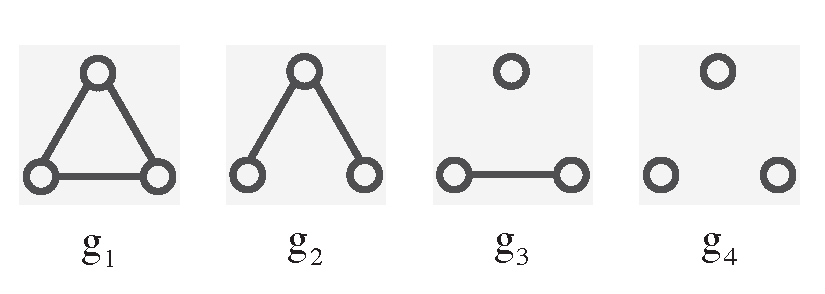
\includegraphics[width =100mm]{3graphlets.pdf}
\caption{Graphlets der Gr\"o"se 3 (\textit{Shervashidze et al.})}
\label{fig:3graphlets}
\end{figure}


\begin{figure}[H]
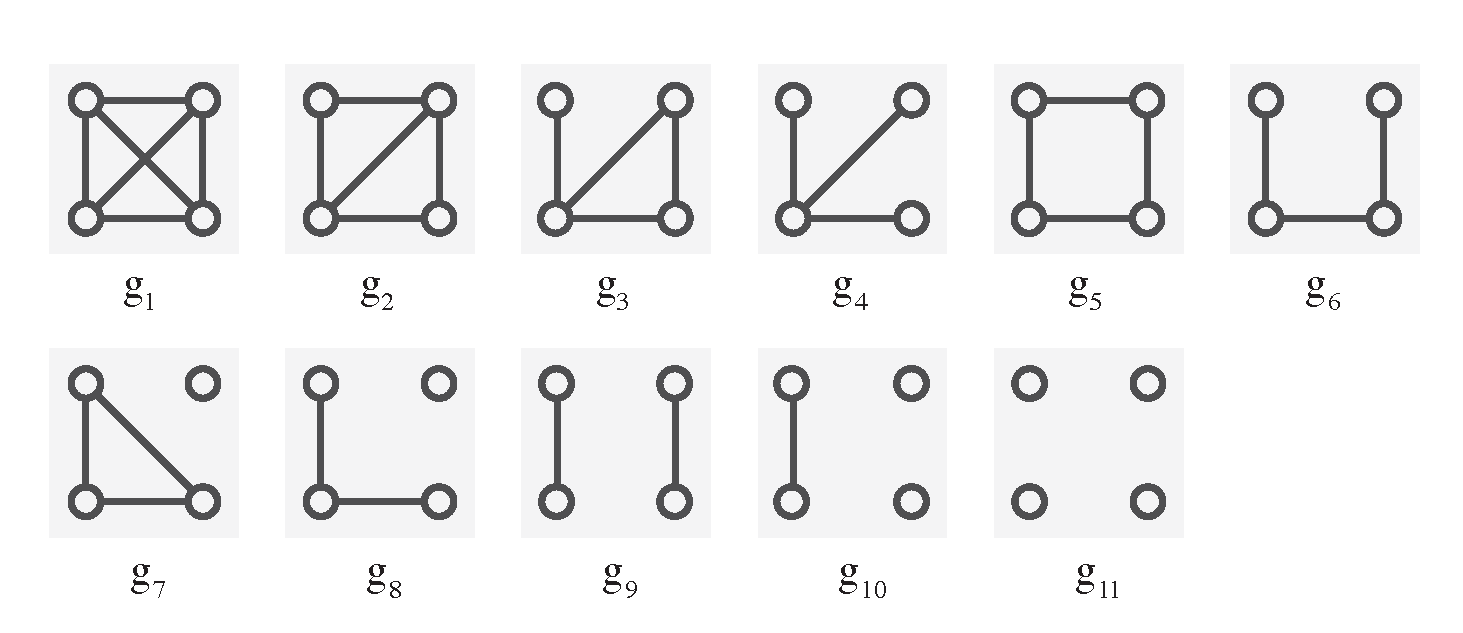
\includegraphics[width =\linewidth]{4graphlets.pdf}
\caption{Graphlets der Gr\"o"se 4 (\textit{Shervashidze et al.})}
\label{fig:4graphlets}
\end{figure}

\end{center}



\begin{figure}[H]
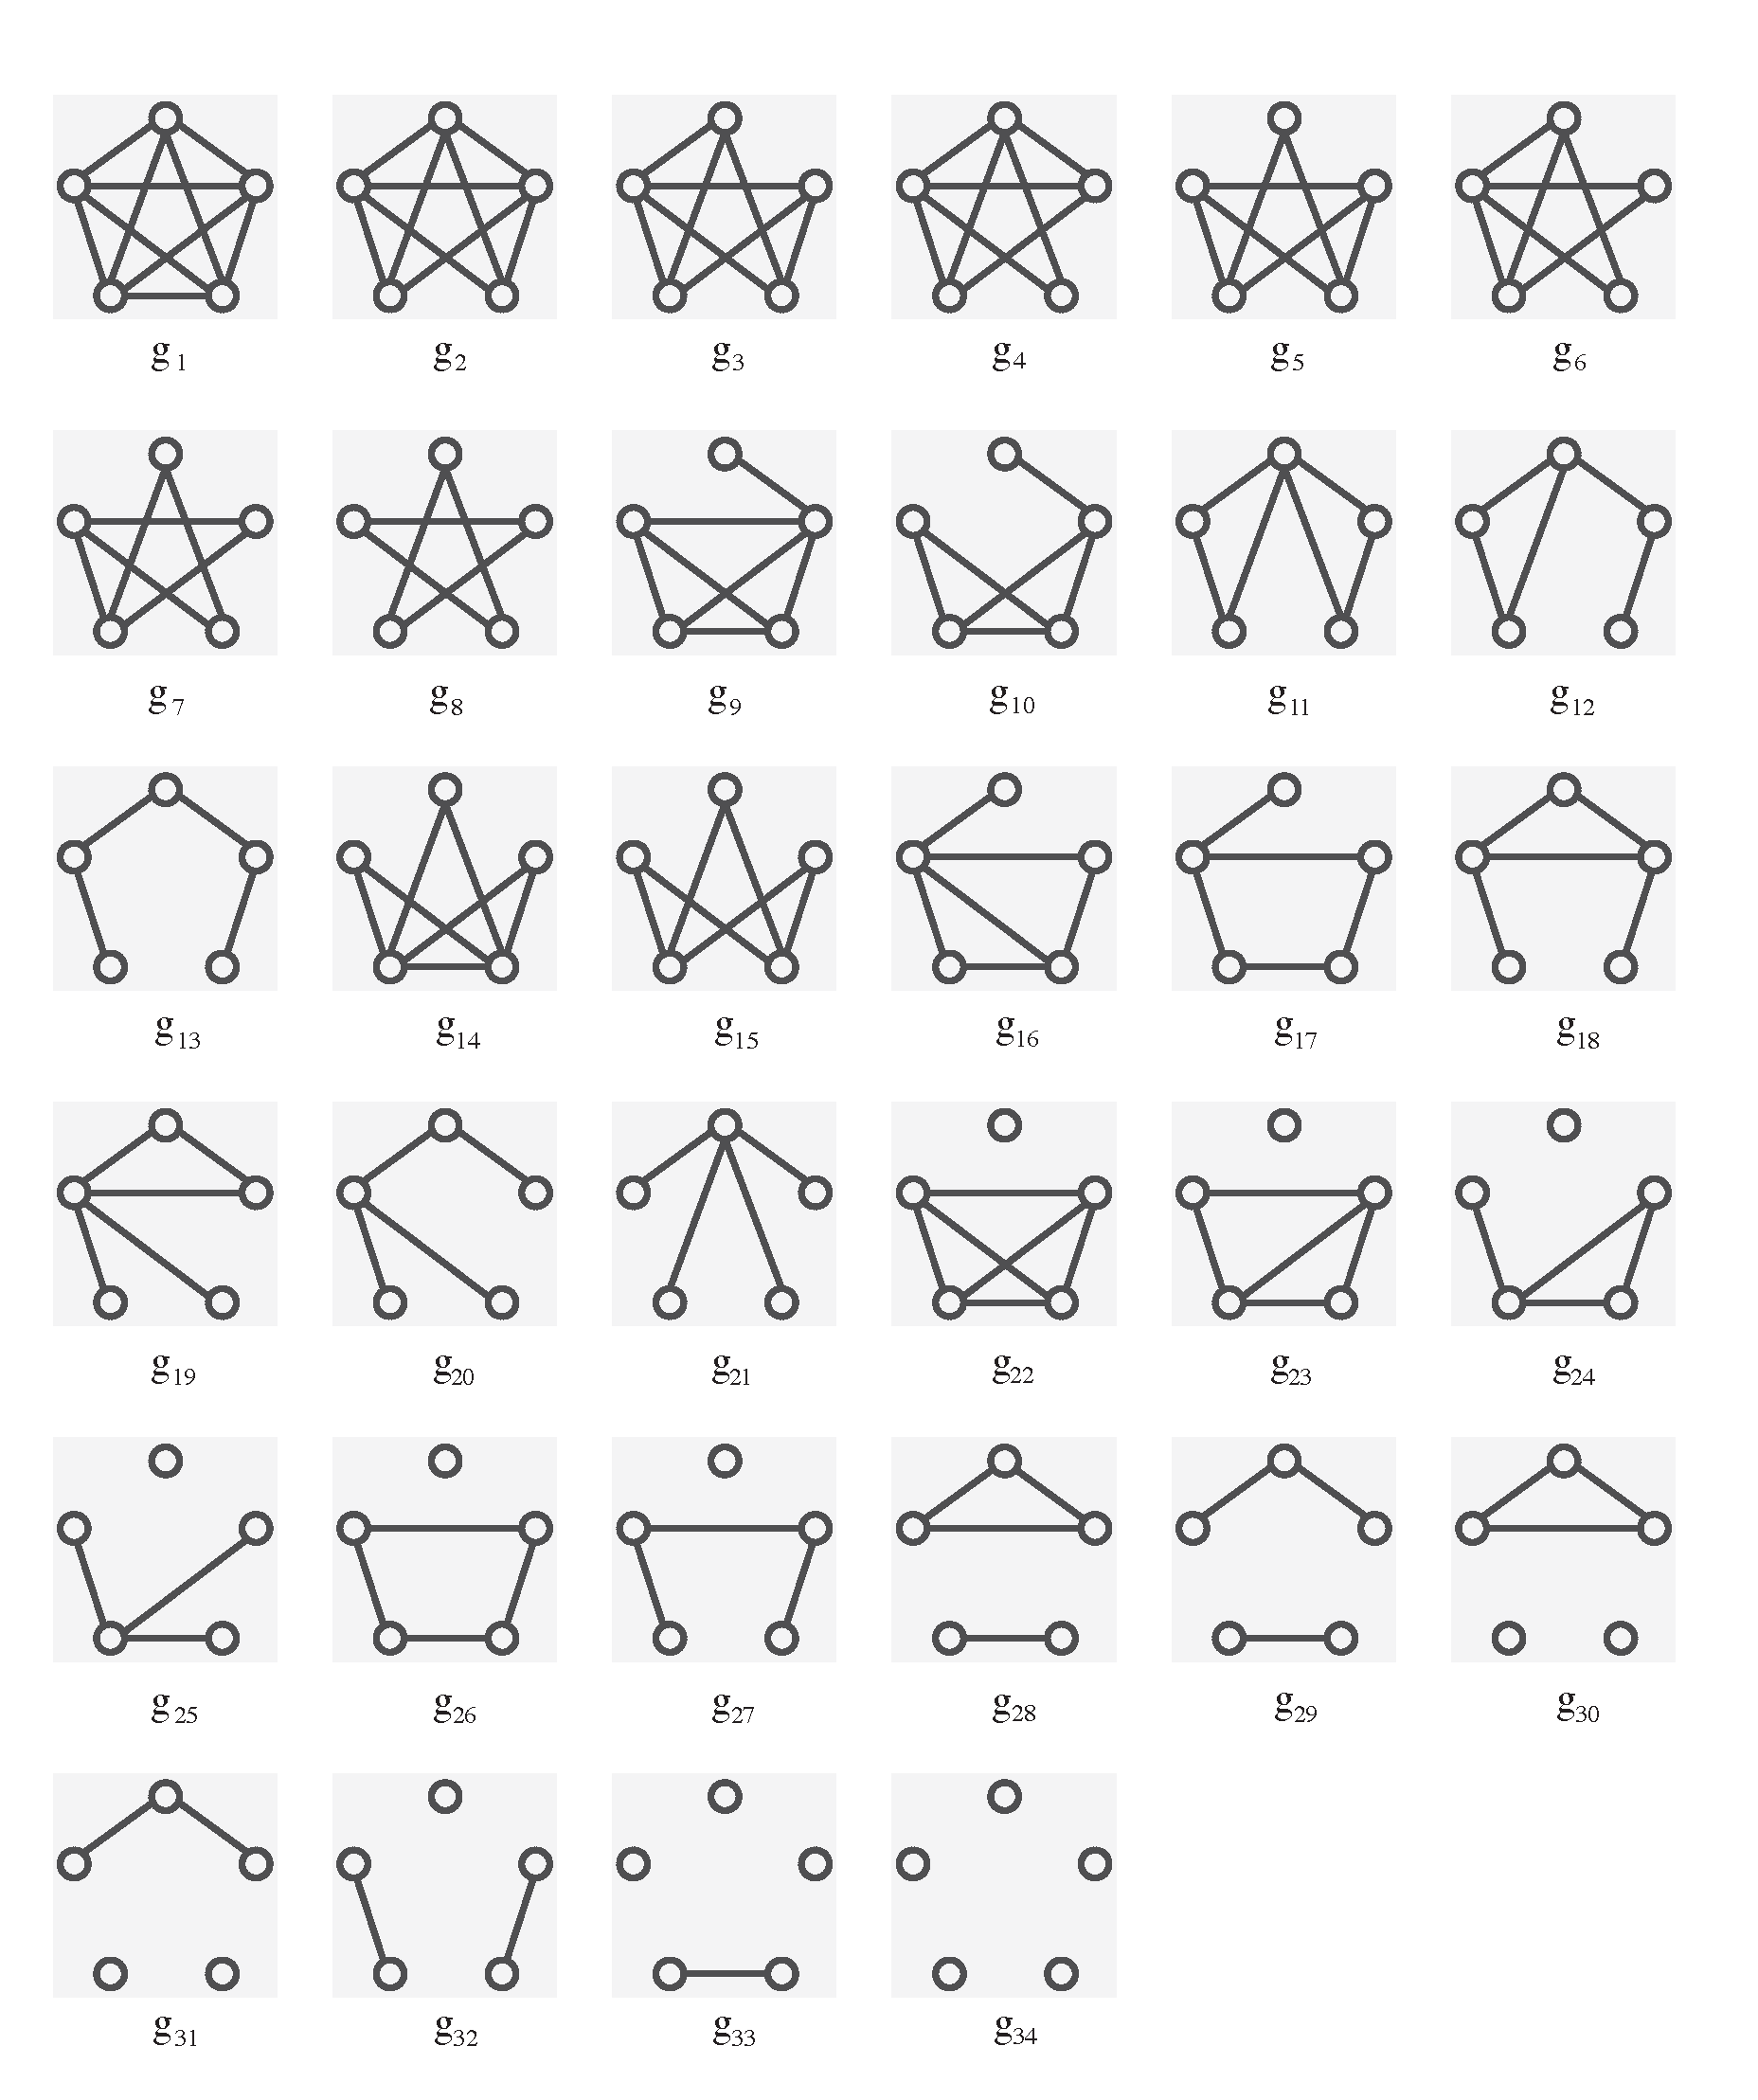
\includegraphics[width =\linewidth]{5graphlets.pdf}
\caption{Graphlets der Gr\"o"se 5 (\textit{Shervashidze et al.})}
\label{fig:5graphlets}
\end{figure}

\newpage

%TODO: UML Diagramm so, konvertieren, dass es eine Bounding Box hat und wieder einf\"ugen

\section{Tabellenverzeichnis}


\begin{table}[H]
\scalebox{0.8}{
\begin{tabular}{l l l l l l l l l l l l l l l l l}

PDB-ID & 1qpu & 1qq3 & 1cgn & 1he9 & 3gf9 & 1exs & 1ngl & 1qqs & 3slo & 1wjx & 5chy & 2id9 & 3i42 & 1d4o & 2w0i &  \\
1qpu &   X   & \cellcolor{fGreen!100}1.139 & \cellcolor{fGreen!75}1.296 & 6.159 & \cellcolor{fGreen!50}5.656 & 10.52 & 11.00 & 12.35 & 12.45 & 11.66 & 7.517 & \cellcolor{fGreen!25}6.128 & 6.625 & 7.326 & 8.572 &  \\
1qq3 & \cellcolor{fGreen!100}1.139 &   X   & \cellcolor{fGreen!75}1.310 & 5.980 & \cellcolor{fGreen!50}5.645 & 9.964 & 10.38 & 11.61 & 11.84 & 11.10 & 6.967 & \cellcolor{fGreen!25}5.776 & 6.039 & 7.491 & 8.059 &  \\
1cgn & \cellcolor{fGreen!100}1.296 & \cellcolor{fGreen!75}1.310 &   X   & 6.093 & \cellcolor{fGreen!25}5.737 & 9.987 & 10.44 & 11.55 & 11.81 & 11.16 & 6.801 & \cellcolor{fGreen!50}5.663 & 5.929 & 7.091 & 7.918 &  \\
1he9 & 6.159 & 5.980 & 6.093 &   X   & \cellcolor{fGreen!100}2.289 & 8.032 & 6.813 & 11.03 & 10.87 & 8.405 & \cellcolor{fGreen!25}3.974 & \cellcolor{fGreen!75}2.445 & \cellcolor{fGreen!50}3.452 & 10.93 & 4.807 &  \\
3gf9 & 5.656 & 5.645 & 5.737 & \cellcolor{fGreen!100}2.289 &   X   & 9.544 & 8.479 & 12.36 & 12.19 & 10.03 & \cellcolor{fGreen!25}5.135 & \cellcolor{fGreen!75}3.370 & \cellcolor{fGreen!50}4.359 & 12.08 & 6.018 &  \\
1exs & 10.52 & 9.964 & 9.987 & 8.032 & 9.544 &   X   & \cellcolor{fGreen!25}4.463 & \cellcolor{fGreen!50}4.041 & \cellcolor{fGreen!75}3.138 & \cellcolor{fGreen!100}2.802 & 4.773 & 7.086 & 5.541 & 7.374 & 4.530 &  \\
1ngl & 11.00 & 10.38 & 10.44 & 6.813 & 8.479 & \cellcolor{fGreen!50}4.463 &   X   & 7.716 & 6.865 & \cellcolor{fGreen!100}3.764 & \cellcolor{fGreen!25}4.718 & 6.054 & 5.065 & 9.755 & \cellcolor{fGreen!75}4.031 &  \\
1qqs & 12.35 & 11.61 & 11.55 & 11.03 & 12.36 & \cellcolor{fGreen!75}4.041 & 7.716 &   X   & \cellcolor{fGreen!100}1.674 & \cellcolor{fGreen!50}5.340 & 8.148 & 10.20 & 8.612 & \cellcolor{fGreen!25}7.226 & 7.404 &  \\
3slo & 12.45 & 11.84 & 11.81 & 10.87 & 12.19 & \cellcolor{fGreen!75}3.138 & \cellcolor{fGreen!25}6.865 & \cellcolor{fGreen!100}1.674 &   X   & \cellcolor{fGreen!50}4.750 & 7.488 & 9.994 & 8.600 & 7.680 & 6.997 &  \\
1wjx & 11.66 & 11.10 & 11.16 & 8.405 & 10.03 & \cellcolor{fGreen!100}2.802 & \cellcolor{fGreen!75}3.764 & 5.340 & \cellcolor{fGreen!25}4.750 &   X   & 5.264 & 7.522 & 5.699 & 8.450 & \cellcolor{fGreen!50}4.384 &  \\
5chy & 7.517 & 6.967 & 6.801 & \cellcolor{fGreen!25}3.974 & 5.135 & 4.773 & 4.718 & 8.148 & 7.488 & 5.264 &   X   & \cellcolor{fGreen!75}2.600 & \cellcolor{fGreen!50}2.817 & 8.667 & \cellcolor{fGreen!100}1.497 &  \\
2id9 & 6.128 & 5.776 & 5.663 & \cellcolor{fGreen!100}2.445 & \cellcolor{fGreen!25}3.370 & 7.086 & 6.054 & 10.20 & 9.994 & 7.522 & \cellcolor{fGreen!50}2.600 &   X   & \cellcolor{fGreen!75}2.447 & 10.24 & 3.657 &  \\
3i42 & 6.625 & 6.039 & 5.929 & \cellcolor{fGreen!25}3.452 & 4.359 & 5.541 & 5.065 & 8.612 & 8.600 & 5.699 & \cellcolor{fGreen!75}2.817 & \cellcolor{fGreen!100}2.447 &   X   & 9.544 & \cellcolor{fGreen!50}2.817 &  \\
1d4o & \cellcolor{fGreen!50}7.326 & 7.491 & \cellcolor{fGreen!100}7.091 & 10.93 & 12.08 & \cellcolor{fGreen!25}7.374 & 9.755 & \cellcolor{fGreen!75}7.226 & 7.680 & 8.450 & 8.667 & 10.24 & 9.544 &   X   & 8.970 &  \\
2w0i & 8.572 & 8.059 & 7.918 & 4.807 & 6.018 & 4.530 & \cellcolor{fGreen!25}4.031 & 7.404 & 6.997 & 4.384 & \cellcolor{fGreen!100}1.497 & \cellcolor{fGreen!50}3.657 & \cellcolor{fGreen!75}2.817 & 8.970 &   X   &  \\



\end{tabular}}
\caption{Distanzen der Aminos\"auregraphen, gemessen mit RGF. In den Zellen der Tabelle stehen die RGF-Distanzen f\"ur die entsprechenden PDB-Dateien. F\"ur jede Zeile (jedes Protein) sind die 4 niedrigsten Distanzen gr\"un unterlegt. Je dunkler das gr\"un ist, desto k\"urzer ist die Distanz.}
\label{table:occ-aag-rgf}
\end{table}



\begin{table}
\scalebox{0.8}{
\begin{tabular}{l l l l l l l l l l l l l l l l l}


PDB-ID & 1qpu & 1qq3 & 1cgn & 1he9 & 3gf9 & 1exs & 1ngl & 1qqs & 3slo & 1wjx & 5chy & 2id9 & 3i42 & 1d4o & 2w0i &  \\
1qpu &   X   & \cellcolor{fGreen!25}0.806 & \cellcolor{fGreen!100}0.606 & \cellcolor{fGreen!50}0.697 & 3.131 & 1.159 & 2.195 & 2.197 & 1.226 & 1.049 & 1.014 & 0.811 & 1.098 & \cellcolor{fGreen!75}0.628 & 0.972 &  \\
1qq3 & \cellcolor{fGreen!25}0.806 &   X   & \cellcolor{fGreen!100}0.405 & 1.504 & 1.567 & 1.703 & 0.883 & 0.883 & 1.396 & 1.270 & 0.869 & \cellcolor{fGreen!75}0.405 & \cellcolor{fGreen!50}0.693 & 0.988 & 1.779 &  \\
1cgn & \cellcolor{fGreen!75}0.606 & \cellcolor{fGreen!100}0.405 &   X   & \cellcolor{fGreen!50}0.810 & 1.432 & 1.633 & 1.193 & 1.193 & 1.513 & 1.339 & 1.060 & \cellcolor{fGreen!25}0.811 & 1.098 & 1.011 & 1.516 &  \\
1he9 & \cellcolor{fGreen!100}0.697 & 1.504 & \cellcolor{fGreen!75}0.810 &   X   & 4.492 & 3.253 & 1.386 & 1.386 & 4.357 & 1.291 & \cellcolor{fGreen!25}1.135 & \cellcolor{fGreen!50}1.099 & 1.386 & 3.599 & 2.506 &  \\
3gf9 & 3.131 & \cellcolor{fGreen!75}1.567 & \cellcolor{fGreen!100}1.432 & 4.492 &   X   & 2.523 & 2.815 & 2.817 & \cellcolor{fGreen!50}1.596 & 2.056 & \cellcolor{fGreen!25}1.816 & 1.917 & 2.034 & 3.122 & 4.130 &  \\
1exs & \cellcolor{fGreen!50}1.159 & 1.703 & 1.633 & 3.253 & 2.523 &   X   & \cellcolor{fGreen!25}1.324 & 1.324 & 2.968 & \cellcolor{fGreen!100}0.696 & \cellcolor{fGreen!75}0.885 & 1.492 & 1.610 & 3.102 & 3.820 &  \\
1ngl & 2.195 & 0.883 & 1.193 & 1.386 & 2.815 & 1.324 &   X   & \cellcolor{fGreen!100}0.002 & \cellcolor{fGreen!50}0.787 & 2.629 & 2.279 & \cellcolor{fGreen!25}0.788 & \cellcolor{fGreen!75}0.286 & 0.980 & 2.722 &  \\
1qqs & 2.197 & 0.883 & 1.193 & 1.386 & 2.817 & 1.324 & \cellcolor{fGreen!100}0.002 &   X   & \cellcolor{fGreen!50}0.787 & 2.631 & 2.281 & \cellcolor{fGreen!25}0.788 & \cellcolor{fGreen!75}0.285 & 0.980 & 2.722 &  \\
3slo & 1.226 & 1.396 & 1.513 & 4.357 & 1.596 & 2.968 & \cellcolor{fGreen!50}0.787 & \cellcolor{fGreen!25}0.787 &   X   & \cellcolor{fGreen!100}0.257 & \cellcolor{fGreen!75}0.705 & 1.024 & 1.073 & 3.137 & 6.154 &  \\
1wjx & 1.049 & 1.270 & 1.339 & 1.291 & 2.056 & \cellcolor{fGreen!50}0.696 & 2.629 & 2.631 & \cellcolor{fGreen!100}0.257 &   X   & 1.043 & 0.933 & \cellcolor{fGreen!25}0.914 & \cellcolor{fGreen!75}0.644 & 2.093 &  \\
5chy & 1.014 & 0.869 & 1.060 & 1.135 & 1.816 & 0.885 & 2.279 & 2.281 & \cellcolor{fGreen!50}0.705 & 1.043 &   X   & \cellcolor{fGreen!75}0.607 & \cellcolor{fGreen!25}0.800 & \cellcolor{fGreen!100}0.275 & 2.282 &  \\
2id9 & 0.811 & \cellcolor{fGreen!100}0.405 & 0.811 & 1.099 & 1.917 & 1.492 & 0.788 & 0.788 & 1.024 & 0.933 & \cellcolor{fGreen!75}0.607 &   X   & \cellcolor{fGreen!50}0.692 & \cellcolor{fGreen!25}0.783 & 2.890 &  \\
3i42 & 1.098 & \cellcolor{fGreen!25}0.693 & 1.098 & 1.386 & 2.034 & 1.610 & \cellcolor{fGreen!75}0.286 & \cellcolor{fGreen!100}0.285 & 1.073 & 0.914 & 0.800 & \cellcolor{fGreen!50}0.692 &   X   & 1.076 & 3.008 &  \\
1d4o & \cellcolor{fGreen!75}0.628 & 0.988 & 1.011 & 3.599 & 3.122 & 3.102 & 0.980 & 0.980 & 3.137 & \cellcolor{fGreen!50}0.644 & \cellcolor{fGreen!100}0.275 & \cellcolor{fGreen!25}0.783 & 1.076 &   X   & 4.406 &  \\
2w0i & \cellcolor{fGreen!100}0.972 & \cellcolor{fGreen!50}1.779 & \cellcolor{fGreen!75}1.516 & 2.506 & 4.130 & 3.820 & 2.722 & 2.722 & 6.154 & \cellcolor{fGreen!25}2.093 & 2.282 & 2.890 & 3.008 & 4.406 &   X   &  \\


\end{tabular}}
\caption{Distanzen der Proteingraphen, gemessen mit RGF. In den Zellen der Tabelle stehen die RGF-Distanzen f\"ur die entsprechenden PDB-Dateien. F\"ur jede Zeile (jedes Protein) sind die 4 niedrigsten Distanzen gr\"un unterlegt. Je dunkler das gr\"un ist, desto k\"urzer ist die Distanz.}
\label{table:occ-pg-rgf}
\end{table}


\begin{table}
\scalebox{0.8}{
\begin{tabular}{l l l l l l l l l l l l l l l l l}

PDB-ID & 1qpu & 1qq3 & 1cgn & 1he9 & 3gf9 & 1exs & 1ngl & 1qqs & 3slo & 1wjx & 5chy & 2id9 & 3i42 & 1d4o & 2w0i &  \\
1qpu &   X   & 4.405 & 5.056 & 2.271 & 10.75 & 3.567 & 2.309 & 13.66 & 14.10 & \cellcolor{fGreen!50}2.128 & \cellcolor{fGreen!75}1.933 & \cellcolor{fGreen!25}2.165 & \cellcolor{fGreen!100}1.877 & 8.791 & 4.422 &  \\
1qq3 & 4.405 &   X   & \cellcolor{fGreen!75}1.906 & \cellcolor{fGreen!100}1.714 & 10.03 & 3.860 & 3.457 & 6.851 & 12.70 & 2.587 & \cellcolor{fGreen!25}2.431 & 2.557 & \cellcolor{fGreen!50}2.269 & 7.907 & 3.002 &  \\
1cgn & 5.056 & 1.906 &   X   & \cellcolor{fGreen!25}0.985 & 9.469 & 1.712 & 1.979 & 7.333 & 12.20 & 1.954 & 1.120 & \cellcolor{fGreen!75}0.249 & \cellcolor{fGreen!100}0.037 & 6.501 & \cellcolor{fGreen!50}0.980 &  \\
1he9 & 2.271 & 1.714 & \cellcolor{fGreen!100}0.985 &   X   & 5.881 & 3.456 & \cellcolor{fGreen!25}1.386 & 4.069 & 5.432 & 1.466 & \cellcolor{fGreen!50}1.291 & \cellcolor{fGreen!75}1.099 & 1.386 & 9.950 & 2.506 &  \\
3gf9 & 10.75 & 10.03 & 9.469 & 5.881 &   X   & 5.473 & 4.230 & 14.86 & 15.99 & \cellcolor{fGreen!75}2.516 & \cellcolor{fGreen!100}1.971 & \cellcolor{fGreen!50}2.575 & \cellcolor{fGreen!25}2.693 & 8.811 & 11.61 &  \\
1exs & 3.567 & 3.860 & 1.712 & 3.456 & 5.473 &   X   & \cellcolor{fGreen!50}1.290 & 3.217 & 4.391 & \cellcolor{fGreen!100}0.611 & \cellcolor{fGreen!75}0.662 & \cellcolor{fGreen!25}1.459 & 1.576 & 9.191 & 4.226 &  \\
1ngl & 2.309 & 3.457 & 1.979 & \cellcolor{fGreen!25}1.386 & 4.230 & \cellcolor{fGreen!50}1.290 &   X   & 3.637 & 2.620 & 2.697 & 2.644 & \cellcolor{fGreen!75}0.788 & \cellcolor{fGreen!100}0.286 & 4.373 & 2.722 &  \\
1qqs & 13.66 & 6.851 & 7.333 & 4.069 & 14.86 & \cellcolor{fGreen!100}3.217 & \cellcolor{fGreen!25}3.637 &   X   & 12.90 & 5.645 & 4.202 & \cellcolor{fGreen!75}3.394 & \cellcolor{fGreen!50}3.512 & 16.22 & 4.907 &  \\
3slo & 14.10 & 12.70 & 12.20 & 5.432 & 15.99 & 4.391 & \cellcolor{fGreen!50}2.620 & 12.90 &   X   & 4.974 & \cellcolor{fGreen!25}3.863 & \cellcolor{fGreen!100}2.351 & \cellcolor{fGreen!75}2.412 & 14.09 & 7.116 &  \\
1wjx & 2.128 & 2.587 & 1.954 & 1.466 & 2.516 & \cellcolor{fGreen!75}0.611 & 2.697 & 5.645 & 4.974 &   X   & \cellcolor{fGreen!100}0.360 & \cellcolor{fGreen!50}0.961 & \cellcolor{fGreen!25}0.965 & 2.225 & 2.042 &  \\
5chy & 1.933 & 2.431 & 1.120 & 1.291 & 1.971 & \cellcolor{fGreen!75}0.662 & 2.644 & 4.202 & 3.863 & \cellcolor{fGreen!100}0.360 &   X   & \cellcolor{fGreen!50}0.797 & \cellcolor{fGreen!25}0.914 & 1.728 & 2.093 &  \\
2id9 & 2.165 & 2.557 & \cellcolor{fGreen!100}0.249 & 1.099 & 2.575 & 1.459 & \cellcolor{fGreen!50}0.788 & 3.394 & 2.351 & 0.961 & \cellcolor{fGreen!25}0.797 &   X   & \cellcolor{fGreen!75}0.692 & 1.921 & 2.890 &  \\
3i42 & 1.877 & 2.269 & \cellcolor{fGreen!100}0.037 & 1.386 & 2.693 & 1.576 & \cellcolor{fGreen!75}0.286 & 3.512 & 2.412 & 0.965 & \cellcolor{fGreen!25}0.914 & \cellcolor{fGreen!50}0.692 &   X   & 2.039 & 3.008 &  \\
1d4o & 8.791 & 7.907 & 6.501 & 9.950 & 8.811 & 9.191 & 4.373 & 16.22 & 14.09 & \cellcolor{fGreen!25}2.225 & \cellcolor{fGreen!100}1.728 & \cellcolor{fGreen!75}1.921 & \cellcolor{fGreen!50}2.039 &   X   & 10.76 &  \\
2w0i & 4.422 & 3.002 & \cellcolor{fGreen!100}0.980 & \cellcolor{fGreen!25}2.506 & 11.61 & 4.226 & 2.722 & 4.907 & 7.116 & \cellcolor{fGreen!75}2.042 & \cellcolor{fGreen!50}2.093 & 2.890 & 3.008 & 10.76 &   X   &  \\



\end{tabular}}
\caption{Distanzen der Komplexgraphen, gemessen mit RGF. In den Zellen der Tabelle stehen die RGF-Distanzen f\"ur die entsprechenden PDB-Dateien. F\"ur jede Zeile (jedes Protein) sind die 4 niedrigsten Distanzen gr\"un unterlegt. Je dunkler das gr\"un ist, desto k\"urzer ist die Distanz.}
\label{table:occ-cg-rgf}
\end{table}



\newpage

\begin{table}
\scalebox{0.8}{
\begin{tabular}{l l l l l l l l l l l l l l l l l}

PDB-ID & 1qpu & 1qq3 & 1cgn & 1he9 & 3gf9 & 1exs & 1ngl & 1qqs & 3slo & 1wjx & 5chy & 2id9 & 3i42 & 1d4o & 2w0i &  \\
1qpu &   X   & \cellcolor{fGreen!75}1.0 & \cellcolor{fGreen!100}1.0 & 0.621 & \cellcolor{fGreen!25}0.666 & 0.276 & 0.25 & 0.25 & 0.224 & 0.25 & 0.538 & \cellcolor{fGreen!50}0.714 & 0.5 & 0.363 & 0.333 &  \\
1qq3 & \cellcolor{fGreen!75}1.0 &   X   & \cellcolor{fGreen!100}1.0 & 0.621 & 0.621 & 0.304 & 0.276 & 0.304 & 0.224 & 0.25 & 0.578 & \cellcolor{fGreen!50}0.666 & \cellcolor{fGreen!25}0.666 & 0.428 & 0.463 &  \\
1cgn & \cellcolor{fGreen!100}1.0 & \cellcolor{fGreen!75}1.0 &   X   & 0.621 & \cellcolor{fGreen!50}0.714 & 0.333 & 0.224 & 0.224 & 0.224 & 0.276 & 0.5 & \cellcolor{fGreen!25}0.666 & 0.578 & 0.333 & 0.428 &  \\
1he9 & 0.621 & 0.621 & 0.621 &   X   & \cellcolor{fGreen!100}0.935 & 0.463 & 0.428 & 0.176 & 0.276 & 0.304 & \cellcolor{fGreen!25}0.621 & \cellcolor{fGreen!75}0.875 & \cellcolor{fGreen!50}0.764 & 0.333 & 0.463 &  \\
3gf9 & \cellcolor{fGreen!25}0.666 & 0.621 & \cellcolor{fGreen!50}0.714 & \cellcolor{fGreen!100}0.935 &   X   & 0.276 & 0.333 & 0.2 & 0.2 & 0.224 & 0.621 & \cellcolor{fGreen!75}0.764 & 0.621 & 0.25 & 0.463 &  \\
1exs & 0.276 & 0.304 & 0.333 & 0.463 & 0.276 &   X   & 0.621 & 0.621 & \cellcolor{fGreen!50}0.764 & \cellcolor{fGreen!100}0.875 & \cellcolor{fGreen!25}0.666 & 0.5 & 0.578 & 0.463 & \cellcolor{fGreen!75}0.818 &  \\
1ngl & 0.25 & 0.276 & 0.224 & 0.428 & 0.333 & \cellcolor{fGreen!50}0.621 &   X   & 0.276 & 0.428 & \cellcolor{fGreen!75}0.666 & \cellcolor{fGreen!25}0.621 & 0.538 & 0.578 & 0.463 & \cellcolor{fGreen!100}0.666 &  \\
1qqs & 0.25 & 0.304 & 0.224 & 0.176 & 0.2 & \cellcolor{fGreen!50}0.621 & 0.276 &   X   & \cellcolor{fGreen!100}1.0 & \cellcolor{fGreen!75}0.621 & \cellcolor{fGreen!25}0.5 & 0.276 & 0.395 & 0.463 & 0.463 &  \\
3slo & 0.224 & 0.224 & 0.224 & 0.276 & 0.2 & \cellcolor{fGreen!75}0.764 & 0.428 & \cellcolor{fGreen!100}1.0 &   X   & \cellcolor{fGreen!50}0.538 & 0.463 & 0.333 & 0.395 & 0.463 & \cellcolor{fGreen!25}0.5 &  \\
1wjx & 0.25 & 0.25 & 0.276 & 0.304 & 0.224 & \cellcolor{fGreen!100}0.875 & \cellcolor{fGreen!75}0.666 & \cellcolor{fGreen!50}0.621 & 0.538 &   X   & 0.538 & 0.363 & 0.5 & 0.395 & \cellcolor{fGreen!25}0.621 &  \\
5chy & 0.538 & 0.578 & 0.5 & 0.621 & 0.621 & \cellcolor{fGreen!25}0.666 & 0.621 & 0.5 & 0.463 & 0.538 &   X   & \cellcolor{fGreen!75}0.818 & \cellcolor{fGreen!50}0.764 & 0.428 & \cellcolor{fGreen!100}1.0 &  \\
2id9 & 0.714 & 0.666 & 0.666 & \cellcolor{fGreen!100}0.875 & \cellcolor{fGreen!25}0.764 & 0.5 & 0.538 & 0.276 & 0.333 & 0.363 & \cellcolor{fGreen!75}0.818 &   X   & \cellcolor{fGreen!50}0.818 & 0.304 & 0.621 &  \\
3i42 & 0.5 & 0.666 & 0.578 & \cellcolor{fGreen!50}0.764 & 0.621 & 0.578 & 0.578 & 0.395 & 0.395 & 0.5 & \cellcolor{fGreen!75}0.764 & \cellcolor{fGreen!100}0.818 &   X   & 0.333 & \cellcolor{fGreen!25}0.714 &  \\
1d4o & 0.363 & 0.428 & 0.333 & 0.333 & 0.25 & \cellcolor{fGreen!25}0.463 & \cellcolor{fGreen!50}0.463 & \cellcolor{fGreen!100}0.463 & \cellcolor{fGreen!75}0.463 & 0.395 & 0.428 & 0.304 & 0.333 &   X   & 0.333 &  \\
2w0i & 0.333 & 0.463 & 0.428 & 0.463 & 0.463 & \cellcolor{fGreen!75}0.818 & \cellcolor{fGreen!25}0.666 & 0.463 & 0.5 & 0.621 & \cellcolor{fGreen!100}1.0 & 0.621 & \cellcolor{fGreen!50}0.714 & 0.333 &   X   &  \\


\end{tabular}}
\caption{Jaccard-Indizes der Aminos\"auregraphen. In den Zellen der Tabelle stehen die Jaccard-Indizes f\"ur die entsprechenden PDB-Dateien. F\"ur jede Zeile (jedes Protein) sind die 4 gr\"o"sten Indizes gr\"un unterlegt. Je dunkler das gr\"un ist, desto gr\"o"ser der Index.}
\label{table:occ-aa-tc}
\end{table}

\begin{table}
\scalebox{0.8}{
\begin{tabular}{l l l l l l l l l l l l l l l l l}

PDB-ID & 1qpu & 1qq3 & 1cgn & 1he9 & 3gf9 & 1exs & 1ngl & 1qqs & 3slo & 1wjx & 5chy & 2id9 & 3i42 & 1d4o & 2w0i &  \\
1qpu &   X   & \cellcolor{fGreen!75}0.764 & \cellcolor{fGreen!100}0.764 & 0.578 & 0.463 & 0.463 & 0.621 & 0.621 & 0.428 & 0.578 & 0.666 & \cellcolor{fGreen!50}0.666 & \cellcolor{fGreen!25}0.666 & 0.538 & 0.395 &  \\
1qq3 & 0.764 &   X   & \cellcolor{fGreen!100}0.935 & 0.764 & 0.463 & 0.621 & 0.714 & 0.714 & 0.538 & 0.714 & \cellcolor{fGreen!25}0.764 & \cellcolor{fGreen!75}0.875 & \cellcolor{fGreen!50}0.818 & 0.666 & 0.5 &  \\
1cgn & \cellcolor{fGreen!25}0.764 & \cellcolor{fGreen!100}0.935 &   X   & 0.764 & 0.428 & 0.578 & 0.714 & 0.714 & 0.538 & 0.666 & 0.714 & \cellcolor{fGreen!75}0.875 & \cellcolor{fGreen!50}0.818 & 0.621 & 0.463 &  \\
1he9 & 0.578 & \cellcolor{fGreen!75}0.764 & \cellcolor{fGreen!100}0.764 &   X   & 0.463 & 0.578 & 0.621 & 0.621 & 0.578 & 0.538 & 0.621 & \cellcolor{fGreen!25}0.714 & \cellcolor{fGreen!50}0.714 & 0.666 & 0.538 &  \\
3gf9 & 0.463 & 0.463 & 0.428 & 0.463 &   X   & 0.428 & \cellcolor{fGreen!25}0.463 & 0.463 & 0.463 & \cellcolor{fGreen!50}0.463 & \cellcolor{fGreen!100}0.538 & 0.428 & 0.463 & \cellcolor{fGreen!75}0.5 & 0.333 &  \\
1exs & 0.463 & \cellcolor{fGreen!25}0.621 & 0.578 & 0.578 & 0.428 &   X   & 0.5 & 0.5 & \cellcolor{fGreen!100}0.714 & 0.5 & 0.578 & \cellcolor{fGreen!50}0.666 & 0.578 & \cellcolor{fGreen!75}0.714 & 0.621 &  \\
1ngl & 0.621 & 0.714 & 0.714 & 0.621 & 0.463 & 0.5 &   X   & \cellcolor{fGreen!100}1.0 & 0.538 & \cellcolor{fGreen!50}0.818 & \cellcolor{fGreen!25}0.818 & 0.818 & \cellcolor{fGreen!75}0.875 & 0.578 & 0.395 &  \\
1qqs & 0.621 & 0.714 & 0.714 & 0.621 & 0.463 & 0.5 & \cellcolor{fGreen!100}1.0 &   X   & 0.538 & \cellcolor{fGreen!25}0.818 & 0.818 & \cellcolor{fGreen!50}0.818 & \cellcolor{fGreen!75}0.875 & 0.578 & 0.395 &  \\
3slo & 0.428 & 0.538 & 0.538 & 0.578 & 0.463 & \cellcolor{fGreen!100}0.714 & 0.538 & 0.538 &   X   & 0.538 & 0.5 & \cellcolor{fGreen!25}0.578 & \cellcolor{fGreen!75}0.621 & \cellcolor{fGreen!50}0.578 & 0.463 &  \\
1wjx & 0.578 & 0.714 & 0.666 & 0.538 & 0.463 & 0.5 & \cellcolor{fGreen!50}0.818 & \cellcolor{fGreen!100}0.818 & 0.538 &   X   & \cellcolor{fGreen!25}0.764 & 0.714 & \cellcolor{fGreen!75}0.818 & 0.538 & 0.395 &  \\
5chy & 0.666 & 0.764 & 0.714 & 0.621 & 0.538 & 0.578 & \cellcolor{fGreen!75}0.818 & \cellcolor{fGreen!25}0.818 & 0.5 & 0.764 &   X   & \cellcolor{fGreen!100}0.875 & \cellcolor{fGreen!50}0.818 & 0.621 & 0.395 &  \\
2id9 & 0.666 & \cellcolor{fGreen!50}0.875 & \cellcolor{fGreen!25}0.875 & 0.714 & 0.428 & 0.666 & 0.818 & 0.818 & 0.578 & 0.714 & \cellcolor{fGreen!75}0.875 &   X   & \cellcolor{fGreen!100}0.935 & 0.714 & 0.463 &  \\
3i42 & 0.666 & 0.818 & 0.818 & 0.714 & 0.463 & 0.578 & \cellcolor{fGreen!50}0.875 & \cellcolor{fGreen!75}0.875 & 0.621 & \cellcolor{fGreen!25}0.818 & 0.818 & \cellcolor{fGreen!100}0.935 &   X   & 0.666 & 0.463 &  \\
1d4o & 0.538 & \cellcolor{fGreen!50}0.666 & 0.621 & 0.666 & 0.5 & \cellcolor{fGreen!100}0.714 & 0.578 & 0.578 & 0.578 & 0.538 & 0.621 & \cellcolor{fGreen!75}0.714 & \cellcolor{fGreen!25}0.666 &   X   & 0.5 &  \\
2w0i & 0.395 & \cellcolor{fGreen!50}0.5 & 0.463 & \cellcolor{fGreen!75}0.538 & 0.333 & \cellcolor{fGreen!100}0.621 & 0.395 & 0.395 & 0.463 & 0.395 & 0.395 & 0.463 & 0.463 & \cellcolor{fGreen!25}0.5 &   X   &  \\

\end{tabular}}
\caption{Jaccard-Indizes der Proteingraphen. In den Zellen der Tabelle stehen die Jaccard-Indizes f\"ur die entsprechenden PDB-Dateien. F\"ur jede Zeile (jedes Protein) sind die 4 gr\"o"sten Indizes gr\"un unterlegt. Je dunkler das gr\"un ist, desto gr\"o"ser der Index.}
\label{table:occ-pg-tf}
\end{table}


\begin{table}
\scalebox{0.8}{
\begin{tabular}{l l l l l l l l l l l l l l l l l}

PDB-ID & 1qpu & 1qq3 & 1cgn & 1he9 & 3gf9 & 1exs & 1ngl & 1qqs & 3slo & 1wjx & 5chy & 2id9 & 3i42 & 1d4o & 2w0i &  \\
1qpu &   X   & \cellcolor{fGreen!100}0.428 & 0.395 & \cellcolor{fGreen!50}0.428 & 0.153 & 0.304 & 0.395 & 0.132 & 0.111 & 0.363 & 0.395 & \cellcolor{fGreen!75}0.428 & \cellcolor{fGreen!25}0.428 & 0.276 & 0.276 &  \\
1qq3 & 0.428 &   X   & \cellcolor{fGreen!100}0.666 & \cellcolor{fGreen!75}0.621 & 0.2 & 0.395 & 0.5 & 0.2 & 0.090 & 0.5 & 0.5 & \cellcolor{fGreen!50}0.538 & \cellcolor{fGreen!25}0.538 & 0.333 & 0.428 &  \\
1cgn & 0.395 & \cellcolor{fGreen!100}0.666 &   X   & \cellcolor{fGreen!75}0.621 & 0.224 & 0.428 & 0.5 & 0.224 & 0.111 & 0.463 & 0.5 & \cellcolor{fGreen!25}0.538 & \cellcolor{fGreen!50}0.538 & 0.363 & 0.363 &  \\
1he9 & 0.428 & 0.621 & 0.621 &   X   & 0.25 & 0.578 & \cellcolor{fGreen!50}0.621 & 0.153 & 0.090 & 0.538 & \cellcolor{fGreen!25}0.621 & \cellcolor{fGreen!100}0.714 & \cellcolor{fGreen!75}0.714 & 0.428 & 0.538 &  \\
3gf9 & 0.153 & 0.2 & 0.224 & 0.25 &   X   & \cellcolor{fGreen!75}0.276 & 0.224 & 0.153 & 0.153 & \cellcolor{fGreen!50}0.276 & \cellcolor{fGreen!100}0.304 & 0.25 & 0.224 & \cellcolor{fGreen!25}0.276 & 0.224 &  \\
1exs & 0.304 & 0.395 & 0.428 & 0.578 & 0.276 &   X   & 0.5 & 0.2 & 0.153 & \cellcolor{fGreen!25}0.578 & 0.578 & \cellcolor{fGreen!100}0.666 & \cellcolor{fGreen!50}0.578 & 0.5 & \cellcolor{fGreen!75}0.621 &  \\
1ngl & 0.395 & 0.5 & 0.5 & 0.621 & 0.224 & 0.5 &   X   & 0.132 & 0.132 & \cellcolor{fGreen!25}0.818 & \cellcolor{fGreen!75}0.818 & \cellcolor{fGreen!50}0.818 & \cellcolor{fGreen!100}0.875 & 0.428 & 0.395 &  \\
1qqs & 0.132 & \cellcolor{fGreen!50}0.2 & \cellcolor{fGreen!100}0.224 & 0.153 & 0.153 & \cellcolor{fGreen!25}0.2 & 0.132 &   X   & \cellcolor{fGreen!75}0.224 & 0.132 & 0.132 & 0.132 & 0.132 & 0.132 & 0.2 &  \\
3slo & 0.111 & 0.090 & 0.111 & 0.090 & \cellcolor{fGreen!25}0.153 & \cellcolor{fGreen!50}0.153 & 0.132 & \cellcolor{fGreen!100}0.224 &   X   & 0.111 & 0.090 & 0.090 & 0.111 & 0.111 & \cellcolor{fGreen!75}0.153 &  \\
1wjx & 0.363 & 0.5 & 0.463 & 0.538 & 0.276 & 0.578 & \cellcolor{fGreen!50}0.818 & 0.132 & 0.111 &   X   & \cellcolor{fGreen!100}0.935 & \cellcolor{fGreen!25}0.714 & \cellcolor{fGreen!75}0.818 & 0.5 & 0.395 &  \\
5chy & 0.395 & 0.5 & 0.5 & 0.621 & 0.304 & 0.578 & \cellcolor{fGreen!25}0.818 & 0.132 & 0.090 & \cellcolor{fGreen!100}0.935 &   X   & \cellcolor{fGreen!75}0.875 & \cellcolor{fGreen!50}0.818 & 0.5 & 0.395 &  \\
2id9 & 0.428 & 0.538 & 0.538 & 0.714 & 0.25 & 0.666 & \cellcolor{fGreen!50}0.818 & 0.132 & 0.090 & \cellcolor{fGreen!25}0.714 & \cellcolor{fGreen!75}0.875 &   X   & \cellcolor{fGreen!100}0.935 & 0.5 & 0.463 &  \\
3i42 & 0.428 & 0.538 & 0.538 & 0.714 & 0.224 & 0.578 & \cellcolor{fGreen!75}0.875 & 0.132 & 0.111 & \cellcolor{fGreen!25}0.818 & \cellcolor{fGreen!50}0.818 & \cellcolor{fGreen!100}0.935 &   X   & 0.428 & 0.463 &  \\
1d4o & 0.276 & 0.333 & 0.363 & 0.428 & 0.276 & \cellcolor{fGreen!100}0.5 & 0.428 & 0.132 & 0.111 & \cellcolor{fGreen!50}0.5 & \cellcolor{fGreen!25}0.5 & \cellcolor{fGreen!75}0.5 & 0.428 &   X   & 0.333 &  \\
2w0i & 0.276 & 0.428 & 0.363 & \cellcolor{fGreen!75}0.538 & 0.224 & \cellcolor{fGreen!100}0.621 & 0.395 & 0.2 & 0.153 & 0.395 & 0.395 & \cellcolor{fGreen!25}0.463 & \cellcolor{fGreen!50}0.463 & 0.333 &   X   &  \\

\end{tabular}}
\caption{Jaccard-Indizes der Komplexgraphen. In den Zellen der Tabelle stehen die Jaccard-Indizes f\"ur die entsprechenden PDB-Dateien. F\"ur jede Zeile (jedes Protein) sind die 4 gr\"o"sten Indizes gr\"un unterlegt. Je dunkler das gr\"un ist, desto gr\"o"ser der Index.}
\label{table:occ-cg-tc}

\end{table}



\bibliographystyle{plain}
\bibliography{literatur}



\end{document}